\documentclass[10pt,twocolumn]{article}

% Pediatric paper draft, derived from main.tex on 2026-09-12 without modifying it.
% Shares references.bib and the generated/ result fragments with main.tex, so the
% pediatric numbers in the \input'ed tables refresh automatically when the
% render jobs listed in main.tex complete.
%
% Provenance rule carried over from main.tex: every numerical value below is
% taken from main.tex, from an audited generated/ fragment, or from a prediction
% file re-derived and verified in PEDS_BENCH. Nothing is estimated.
%
% Two pediatric protocols appear. The frozen MRN-disjoint <18 test split
% (N=1,273) is PRIMARY. The historical age>=5 validation cohort (N=1,507) is a
% REPLICATION cohort and is never described as a sealed test set. All <18
% results currently come from the 20:00 checkpoint snapshot while training
% continues; they are labelled interim wherever they appear.
\usepackage[margin=0.68in,columnsep=0.22in]{geometry}
\usepackage[T1]{fontenc}
\usepackage{lmodern}
\usepackage{microtype}
\usepackage{booktabs}
\usepackage{multirow}
\usepackage{makecell}
\usepackage{tabularx}
\usepackage{threeparttable}
\usepackage{amsmath,amssymb}
\usepackage{graphicx}
\usepackage{xcolor}
\usepackage{tikz}
\usetikzlibrary{arrows.meta,positioning,fit,backgrounds}
\usepackage{pgfplots}
\pgfplotsset{compat=1.18}
\usepackage{hyperref}
\usepackage[capitalize,noabbrev]{cleveref}
\usepackage{enumitem}
\setlist{nosep,leftmargin=*}

% ---- Float and table layout for a dense two-column paper ----------------
% In twocolumn mode a table* may only sit at the top of a page and never before
% its source position, so a long run of wide tables queues and dumps after the
% bibliography. dblfloatfix lets double-column floats also go to the page
% bottom and keeps their order; the relaxed fractions let text pages carry more
% float area; \clearpage before \appendix flushes the main-text queue there.
\usepackage{dblfloatfix}
\setcounter{topnumber}{4}\setcounter{bottomnumber}{3}\setcounter{totalnumber}{6}
\setcounter{dbltopnumber}{3}
\renewcommand{\topfraction}{0.95}\renewcommand{\bottomfraction}{0.9}
\renewcommand{\dbltopfraction}{0.95}\renewcommand{\textfraction}{0.05}
\renewcommand{\floatpagefraction}{0.85}\renewcommand{\dblfloatpagefraction}{0.85}
% Float-only pages centre their floats vertically by default, which left the
% wide retrieval table stranded mid-page with blank space above it.
\makeatletter\setlength{\@fptop}{0pt}\setlength{\@dblfptop}{0pt}
\setlength{\@fpbot}{0pt plus 1fil}\setlength{\@dblfpbot}{0pt plus 1fil}
% The separation between floats on a float page is rubber by default, which
% stretched into a half-page gap between the two appendix tables.
\setlength{\@fpsep}{20pt}\setlength{\@dblfpsep}{20pt}\makeatother
% All tabular material in \small, including the auto-generated fragments, which
% cannot be edited in place; this alone removes the 5-30pt overfull cases.
\usepackage{etoolbox}
\AtBeginEnvironment{tabular}{\small}
\AtBeginEnvironment{tabularx}{\small}

\definecolor{ctblue}{HTML}{3977B7}
\definecolor{ctxorange}{HTML}{E68A2E}
\definecolor{ctxgreen}{HTML}{2A9D6F}
\definecolor{lightgray}{HTML}{F2F3F5}
\newcommand{\ours}{\textsc{MetaQ-CT}}
\newcommand{\todo}[1]{\textcolor{red}{[TODO: #1]}}
\newcommand{\best}[1]{\textbf{#1}}

\title{Clinical Context Matters: Metadata-Conditioned\\
Vision--Language Modeling for Pediatric Chest CT}
\author{Anonymous Authors}
\date{}

\begin{document}
\maketitle

\begin{abstract}
Vision--language models for chest CT are trained and benchmarked almost
exclusively on adult cohorts, and they read a volume with generic pathology
prompts even though the clinical indication, age, and sex that motivated the
examination are available at interpretation time. Both choices are costly in
pediatric radiology, where anatomy, disease priors, and reconstruction
geometry differ from adults and where indications are unusually informative.
We present \ours, a metadata-conditioned Q-Former on an anatomy-routed 3-D CT
encoder that retains a metadata-independent query bank while adding
pathology-specific conditioned queries attending to indication, age, and sex
through gated cross-attention and identity-initialized feature-wise
modulation. On a frozen, MRN-disjoint pediatric test split of 1,273 studies
spanning ages 0--18 and 23 findings, conditioning improves three-seed macro
AUROC from 0.7687 to 0.8268 ($\Delta=+0.0581$, patient-bootstrap 95\% CI
[0.0482, 0.0685], $p<0.001$) and macro AUPRC from 0.3592 to 0.4616, with a
positive gain in every prespecified age bin, both sexes, both examination-year
strata, and all four prespecified high-volume acquisition-site strata. A historical age-$\geq5$ validation
cohort of 1,507 studies replicates the effect ($0.7933\pm0.0017$ to
$0.8396\pm0.0015$), and blanking or shuffling indications there returns
AUROC to 0.8092 and 0.7960, so the gain depends on the \emph{correct} patient
context. A no-CT control shows that indication text alone already reaches
0.7860. The multimodal model exceeds both it and the matched CT-only model.
Finally, a locally measured benchmark of ten methods on the same pediatric
cohort shows that released adult CT foundation models transfer poorly to
children. A 2-D biomedical encoder with a linear probe outperforms every
volumetric CT model we could reproduce. This underscores why pediatric
performance must be measured rather than inherited from adult tables.
\end{abstract}

\section{Introduction}
Volumetric chest CT vision--language systems such as
CT-CLIP~\cite{hamamci2024ctclip}, MPS-CT~\cite{li2025mpsct},
GreenRFM~\cite{li2026greenrfm}, and ARC-CT~\cite{isik2026arcct} have raised
adult abnormality-classification performance rapidly, largely on the CT-RATE
benchmark. Two properties of that progress do not carry into pediatric
practice. First, the models are trained on adults and evaluated on adults.
Pediatric anatomy is smaller, disease prevalence is different, and thin-slice
reconstruction geometry differs. No public pediatric chest-CT benchmark exists
against which transfer can be checked. Second, the standard readout is
a positive/negative pathology-prompt softmax that ignores the clinical
question. In pediatric radiology that question is seldom generic: indications
encode malignancy history, transplant status, postoperative context, cystic
fibrosis surveillance, or a focused diagnostic concern, and they alter disease
priors substantially before a single voxel is examined.

A naive remedy is to concatenate a global metadata embedding to the image
embedding. That remedy imposes the same correction on unrelated pathologies, so
helpful and harmful effects can cancel. We instead condition pathology-specific
query slots on clinical context while preserving a separate, metadata-free
general representation, so that the model can benefit from the indication for
the pathologies it concerns and leave the rest untouched.

This paper makes four contributions specific to pediatric chest CT:
\begin{itemize}
    \item a metadata-conditioned Q-Former that combines pathology-specific
    clinical cross-attention, identity-initialized FiLM, and a class-specific
    clinical-relevance gate, built on an anatomy-routed 3-D encoder.
    \item a frozen, MRN-disjoint pediatric evaluation protocol covering ages
    0--18 with 23 pediatric-relevant findings, three seeds per arm,
    patient-bootstrap confidence intervals, and prespecified age, sex,
    examination-year, and site subgroups. It is replicated on a second
    historical pediatric cohort.
    \item causal and leakage controls that separate genuine visual--clinical
    fusion from text-only shortcuts. The controls are correct versus blank
    versus shuffled indications, no-CT metadata-only heads, and stratification
    by explicit target terminology in the indication.
    \item the first locally measured pediatric benchmark of released chest-CT
    foundation models, showing how far adult rankings fail to transfer and
    which model families degrade most.
\end{itemize}

\section{Method}
\Cref{fig:architecture} gives an overview of the model. The following
subsections define each component.

\subsection{Base volumetric representation}
Given a CT volume $X$, an R(2+1)D-18 encoder produces a 512-channel spatial
feature map. The encoder starts from Kinetics weights and is first adapted for
eight epochs on the 23 pediatric labels with asymmetric multilabel loss. The
checkpoint with the highest development macro AUROC initializes Stage 2. Thus,
the primary $<18$ experiment follows the ARC-CT anatomy-query design but does
\emph{not} load an adult ARC-CT checkpoint. Its transferable priors are the
Kinetics visual initialization and pretrained biomedical language encoders.

Stage 2 uses a four-layer, eight-head, 768-dimensional anatomy-aware Q-Former.
For $C$ pathology targets, the general bank contains 10 anatomy queries, $C$
pathology queries, and two global queries. Its pooled representation
$z_{\mathrm{gen}}$ is deliberately isolated from metadata-conditioned slots,
retaining a canonical metadata-free image/report embedding. The 10 pediatric
regions are the five lung lobes, central airway and esophagus, heart and great
vessels, pleural space, chest wall and skeleton, and upper abdomen. All 6,341
studies in the primary splits have a matched TotalSegmentator-derived mask.
The primary recipe requires that mask and restricts each anatomy query to its
assigned region. Mask-free operation is a registered ablation rather than a
silent fallback.

\subsection{Clinical context encoder}
The clinical context combines indication text $I$, a learned age
representation $a$, sex $s$, and an age--sex interaction:
\begin{equation}
H_C = \operatorname{ContextEncoder}(I,a,s).
\end{equation}
The indication is tokenized to at most 64 tokens and encoded as a \emph{token
sequence}, rather than a single pooled vector, by a separate frozen
CXR-BERT. Three learned 768-dimensional demographic tokens are appended: age,
sex, and their interaction. Age first enters a 64-dimensional ordinal
embedding, sex a 16-dimensional embedding with female, male, and unknown rows,
and their interaction a 32-dimensional table. Separate linear projections map
all three to the Q-Former width. The interaction table and its projection start
at zero so that an age--sex interaction is learned only when supported by data.

The age representation is an ordered cumulative embedding,
\begin{equation}
e_{\mathrm{age}}(b)=e_0+\sum_{j < b}\operatorname{softplus}(\delta_j),
\end{equation}
which enforces band order while allowing the distance between adjacent bands
to be learned. The complete shared vocabulary contains 10 half-open bands:
$[0,1)$, $[1,2)$, $[2,5)$, $[5,10)$, $[10,13)$, $[13,18)$, $[18,25)$,
$[25,40)$, $[40,60)$, and $[60,\infty)$ years, plus a separate unknown row.
Only the first six occur in the primary pediatric cohort. This is distinct
from the five wider age bins used only for subgroup reporting.

Missing or unusable indications are represented by the single canonical text
``no clinical indication provided.'' Age and sex have explicit unknown rows
and are never imputed from other patients. The primary arm randomly replaces
30\% of training indications with the canonical missing string, while retaining
age and sex, to prevent brittle dependence on text. No indication dropout is
applied at evaluation. The historical replication checkpoints used scalar age
and 10\% indication dropout.

\begin{table*}[t]
\centering
\caption{Illustrative model inputs. Indications are paraphrased composites,
not verbatim patient records. They demonstrate the clinical information
available to the model without disclosing protected health information.}
\label{tab:context-examples}
\begin{tabularx}{\textwidth}{@{}ll>{\hsize=1.3\hsize}X>{\hsize=0.85\hsize}X>{\hsize=0.85\hsize}X@{}}
\toprule
Age band & Sex token & Paraphrased indication & Information conveyed & Candidate affected findings \\
\midrule
$[0,1)$ & female & Postoperative congenital heart disease; new respiratory distress & Surgical context and acute change & medical material, atelectasis, effusion \\
$[2,5)$ & male & Treated solid tumour; surveillance for pulmonary spread & Oncologic history and purpose of examination & pulmonary metastases, nodules \\
$[5,10)$ & female & Cystic-fibrosis follow-up; assess airway disease & Chronic diagnosis and targeted question & bronchiectasis, mucus plugging \\
$[13,18)$ & male & Fever after stem-cell transplantation; evaluate opportunistic infection & Immunosuppression and acute symptom & nodules, opacity, consolidation \\
unknown & unknown & no clinical indication provided & Explicit missingness, not fabricated text & no class-specific textual prior \\
\bottomrule
\end{tabularx}
\end{table*}

\subsection{C1: pathology-specific conditioning}
Each general pathology query has a conditioned twin. The conditioned query
attends to $H_C$ through a gated cross-attention residual and is then modulated
by FiLM:
\begin{align}
\widetilde q_c &= q_c + g_c\,
  \operatorname{CrossAttn}(q_c,H_C),\\
q^{\mathrm{ind}}_c &= \gamma_c(H_C)\odot \widetilde q_c + \beta_c(H_C).
\end{align}
The modulation is initialized near identity ($\gamma\approx1$,
$\beta\approx0$), so the pretrained CT pathway remains stable early in
adaptation. A clinical/global conditioned slot is added alongside the $C$
pathology twins, giving $13+2C=59$ slots for the 23-class pediatric task.

\subsection{C2: class-specific clinical relevance}
For each pathology $c$, C2 compares the indication embedding $e_I$ with a
frozen class-prompt embedding $p_c$:
\begin{align}
r_c &= \sigma\!\left(\operatorname{MLP}
  [e_I;p_c;e_I\odot p_c]\right),\\
w_c &= 1+\operatorname{softplus}(b)r_c.
\end{align}
The non-negative weight $w_c$ controls conditioned-pathology pooling and the
conditioned prompt loss. With $b=-2$ at initialization, C2 starts as a modest
correction and can never push an incidental finding below its unconditioned
weight.

\subsection{Fusion and readouts}
The primary model pools the $C$ conditioned pathology twins with C2 weights
and averages that representation with the clinical/global slot:
\begin{align}
z_{\mathrm{pool}} &= \frac{\sum_c w_c t_c^{\mathrm{ind}}}{\sum_c w_c}, &
z_{\mathrm{ind}} &= \tfrac12(z_{\mathrm{pool}}+z_{\mathrm{clin}}),\\
z_{\mathrm{final}} &= W_f[z_{\mathrm{gen}};z_{\mathrm{ind}}], &
W_f &\leftarrow [I\;0].
\end{align}
Both branches use the same positive/negative pathology-prompt softmax. The
general branch reads $z_{\mathrm{gen}}$ and the conditioned branch reads
$z_{\mathrm{final}}$. Because $W_f$ starts as $[I\;0]$ and every conditioning
path is zero-gated or identity-initialized, the conditioned readout equals the
general readout at step zero. Everything the conditioned branch learns is
therefore a departure from the CT-only parent. A separate supervised
\texttt{ctx\_cls} head (LayerNorm plus one linear layer on
$[z_{\mathrm{gen}};z_{\mathrm{ind}}]$) is evaluated only as a labeled ablation
and never conflated with prompt inference.

\subsection{Training objective}
Stage 1 trains the Kinetics-initialized R(2+1)D-18 encoder and a temporary
23-output linear head with asymmetric loss for eight epochs (batch size 8,
learning rate $10^{-4}$, weight decay $10^{-4}$). The head is discarded after
development selection. Stage 2 loads the selected visual encoder and jointly
optimizes the image pathway, Q-Former, visual/text projections, CXR-BERT LoRA
parameters, and the new context modules. It uses batches of four with eight
gradient-accumulation steps, at most 10,000 optimizer updates, a 500-update
warm-up, and development evaluation every 500 updates. The base vision learning
rate is $10^{-5}$, the text learning rate $10^{-7}$, and the zero-initialized
context modules use a $20\times$ multiplier. Base and context gradient norms
are clipped separately.

The Stage-2 pediatric recipe optimizes
\begin{equation}
\mathcal{L}=\mathcal{L}_{\mathrm{clip}}
+0.5\mathcal{L}_{\mathrm{prompt}}
+0.5\mathcal{L}_{\mathrm{align}}
+0.5\mathcal{L}_{\mathrm{ptok}}
+2.0\mathcal{L}_{\mathrm{ind}},
\end{equation}
where $\mathcal{L}_{\mathrm{clip}}$ aligns whole-volume and report embeddings,
$\mathcal{L}_{\mathrm{prompt}}$ is the general multilabel prompt loss,
$\mathcal{L}_{\mathrm{align}}$ aligns anatomy-pooled image features with
organ-localized findings text, $\mathcal{L}_{\mathrm{ptok}}$ supervises
pathology tokens, and $\mathcal{L}_{\mathrm{ind}}$ is the conditioned prompt
loss. Training uses temperature one, null/empty negative prompts, no L2
normalization, and checkpoint selection by conditioned development AUROC.
The counterfactual loss and auxiliary \texttt{ctx\_cls} loss are zero in the
primary arm and appear only in named ablations. No CT-RATE scan enters a
pediatric minibatch, and no pediatric test study participates in optimization
or checkpoint selection.

\begin{figure*}[t]
\centering
%% PLACEHOLDER: the real architecture figure is being redrawn; blank space is
%% reserved here. The original TikZ source is kept in
%% figures/_pipeline_figures_original.tex and can be pasted back verbatim.
\vspace*{4.6cm}
\caption{Architecture for the 23-finding pediatric task. The
metadata-independent general bank is retained. Pathology-specific conditioned
twins attend to clinical context through C1 cross-attention and FiLM and are
pooled by C2 relevance weights. Prompt inference is the primary readout.
\texttt{ctx\_cls} is a separate supervised ablation.}
\label{fig:architecture}
\end{figure*}

\section{Pediatric Cohort and Protocol}
\subsection{Source archive, eligibility, and privacy}
The retrospective source archive contains 8,870 chest-CT report records from a
single children's hospital. Existing conversion and quality-control filters
produced 8,760 model-ready thin-slice volumes. The present paper then retained
the 6,341 examinations acquired at $0\leq$age$<18$. The examinations span
2011--2026 and are non-contrast chest CTs. Every included study has a volume,
report, 23-label vector, clinical-context row, and anatomy mask. No included
study is silently dropped for missing imaging or segmentation.

Raw identifiers are used only inside the institutional computing environment
to establish the MRN-level split. Model-facing tables are keyed by a
de-identified volume identifier. The indication is parsed from the report,
then scrubbed against row-specific patient identifiers, accession numbers,
dates, a cohort-wide patient/provider name pool, and structural identifier
patterns. Fatal preflight checks reject surviving MRNs, accessions, long digit
strings, dates, contact information, duplicate keys, or incomplete split
coverage. Report and indication processing is performed locally. Clinical
text is not sent to an external service.

\begin{figure*}[t]
\centering
%% PLACEHOLDER: the real cohort-flow figure is being redrawn; blank space is
%% reserved here. The original TikZ source is kept in
%% figures/_pipeline_figures_original.tex and can be pasted back verbatim.
\vspace*{4.0cm}
\caption{Assembly of the primary pediatric cohort. Train, development, and
test are mutually exclusive at the MRN/patient level. The historical source
validation pool is retained as the frozen test cohort. The source training
pool alone is divided into train and development.}
\label{fig:cohort-flow}
\end{figure*}

\subsection{Report-derived label construction}
Findings and impression sections are divided into numbered sentences and
processed locally by Qwen3-8B under constrained JSON decoding. For each of 27
candidate findings, the extractor returns a binary decision and the index of
the supporting report sentence. Out-of-range indices and malformed records are
detectable failures rather than silent all-zero labels. The paper task removes
four adult-specific or inadequately supported targets from both training and
evaluation, leaving 23 outputs. The removed targets are arterial wall
calcification, coronary artery calcification, hiatal hernia, and emphysema. The labels are therefore
report-derived weak supervision, not independent image adjudications.

The full findings text is encoded during Stage 2 for global image--report
alignment. Organ-specific text for the primary run is selected from the
findings section by anatomy-keyword matching. The available Qwen organ-sentence
cache is a named ablation and is not used in the primary result. Reports are
training supervision only: at inference the model receives the CT, scrubbed
indication, age band, sex, and fixed pathology prompts, but never the report
whose findings define the reference labels.

\subsection{CT and anatomy preprocessing}
Volumes are stored in Hounsfield units and deterministically padded or cropped
to $192\times192\times96$ voxels, with out-of-field values clamped to the
$-1024$ HU air floor before padding. Three channels encode lung, soft-tissue,
and bone windows. Stage 1 uses a lung window of $[-1500,500]$ HU and Stage 2 uses
$[-1000,400]$ HU. Both use $[-160,240]$ and $[300,2000]$ HU for soft tissue
and bone. Training augmentation pads to $240\times240\times120$ before
a paired random image/mask crop, permits anatomy-preserving flips, and applies
HU intensity jitter (30 HU in Stage 1 and 20 HU in Stage 2). Evaluation uses
the deterministic center geometry.

TotalSegmentator structures are merged into the 10 pediatric regions used by
the anatomy queries. Distributed targets such as medical material,
lymphadenopathy, post-treatment change, and mass/neoplasm remain unrestricted
rather than being assigned a confidently wrong region. Image and mask undergo
identical spatial transforms.

\subsection{Two evaluation protocols}
\Cref{tab:cohorts} summarizes the two pediatric protocols used in this paper.

\paragraph{Frozen $<18$ protocol (primary).}
Every study with $0\leq$age$<18$ is retained, including ages 0--5. The
historical training pool was divided by medical record number (MRN) into
4,320 training studies (2,108 patients) and 748 development studies (373
patients). The historical patient-disjoint validation pool contributes 1,273
test studies (611 patients). Patient overlap is zero for every pair of splits.
Because this source test pool was inspected during earlier exploratory work,
we describe it as a \emph{frozen retrospective} test rather than a
never-observed prospective one.

\paragraph{Historical age-$\geq5$ protocol (replication).}
An earlier campaign excluded examinations below age five and used 5,948
training and 1,509 validation studies with patient-disjoint splitting. An
MRN-level audit confirmed no patient overlap between those pools. The same
audit found that the 1,507 scored studies were contained in the 1,509-study
Stage-2 model-selection validation list. We therefore label every result on
this cohort as historical held-out \emph{validation}, never as sealed test
performance, and use it as a replication cohort for the frozen protocol.

\begin{table*}[t]
\centering
\caption{Pediatric cohorts and matched experimental splits.}
\label{tab:cohorts}
\begin{tabular}{@{}lrrrrp{5.2cm}@{}}
\toprule
Protocol & Train & Development & Test / validation & Classes & Provenance \\
\midrule
Frozen $<18$ (primary) & 4,320 & 748 & 1,273 & 23 & MRN-disjoint train/development/test; includes ages 0--5; 2,108 / 373 / 611 patients \\
Historical age-$\geq5$ (replication) & 5,948 & 1,509 & N/A & 23 & Patient-disjoint train/validation; the 1,507 scored studies (648 patients) are a subset of the model-selection validation pool \\
\bottomrule
\end{tabular}
\end{table*}

\paragraph{Unfiltered all-age sensitivity cohort.}
To measure the joint effect of retaining both children younger than five and
patients who have reached adulthood, we additionally use every study in the
clean source split without an age cutoff. This cohort spans 0.01--69 years and
contains 7,001 training studies from 3,180 patients and 1,761 validation
studies from 791 patients, with zero MRN or study overlap. Its Stage-1 encoder
is retrained on the same all-age training pool, followed by three full-model
and three matched CT-only Stage-2 seeds. Quantitative results will enter the
paper only after all six paired evaluations complete.

\begin{table*}[t]
\centering
\caption{Characteristics of the primary MRN-disjoint pediatric cohort. Word
counts refer to present indications and to the de-identified findings section,
respectively. Percentages use studies, not patients, as the denominator.}
\label{tab:cohort-characteristics}
\begin{tabular}{@{}lrrrr@{}}
\toprule
Characteristic & Train & Development & Frozen test & All \\
\midrule
Studies & 4,320 & 748 & 1,273 & 6,341 \\
Patients & 2,108 & 373 & 611 & 3,092 \\
Age, mean $\pm$ SD (years) & $10.19\pm5.23$ & $9.96\pm5.31$ & $10.17\pm5.11$ & $10.16\pm5.22$ \\
Age, median [IQR] (years) & 11 [6--15] & 11 [5--15] & 11 [6--15] & 11 [6--15] \\
Female, $n$ (\%) & 1,941 (44.93) & 358 (47.86) & 681 (53.50) & 2,980 (47.00) \\
Male, $n$ (\%) & 2,372 (54.91) & 390 (52.14) & 592 (46.50) & 3,354 (52.89) \\
Unknown sex, $n$ (\%) & 7 (0.16) & 0 & 0 & 7 (0.11) \\
Indication present, $n$ (\%) & 4,303 (99.61) & 746 (99.73) & 1,269 (99.69) & 6,318 (99.64) \\
Indication words, median [IQR] & 22 [16--31] & 22 [16--32] & 22 [16--31] & 22 [16--31] \\
Findings words, median [IQR] & 156 [114--214] & 147 [110--208] & 158 [117--212] & 156 [114--213] \\
Zero positive targets, $n$ (\%) & 418 (9.68) & 52 (6.95) & 120 (9.43) & 590 (9.30) \\
Positive targets/study, mean (median) & 3.26 (3) & 3.23 (3) & 3.25 (3) & 3.26 (3) \\
Matched CT and anatomy mask, $n$ (\%) & 4,320 (100) & 748 (100) & 1,273 (100) & 6,341 (100) \\
\bottomrule
\end{tabular}
\end{table*}

\begin{figure*}[t]
\centering
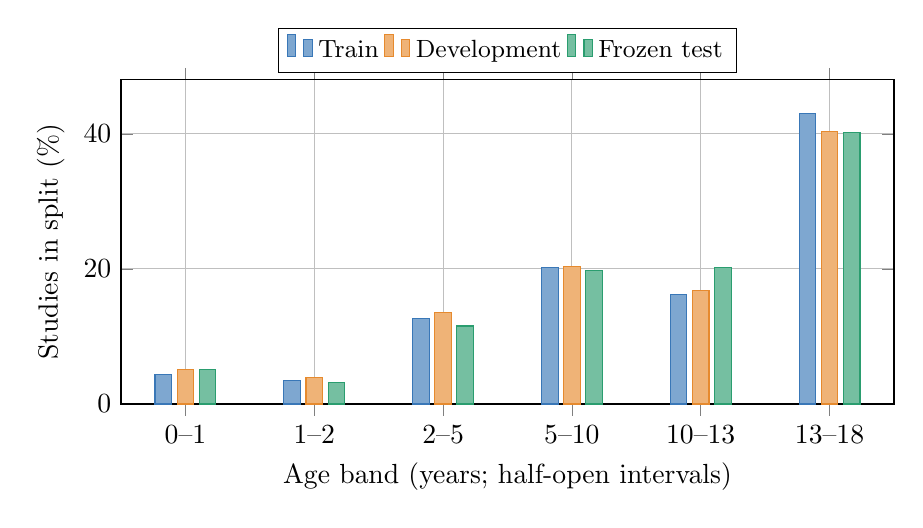
\begin{tikzpicture}
\begin{axis}[
  width=0.94\textwidth,height=5.7cm,
  ybar,bar width=6pt,
  ylabel={Studies in split (\%)},
  xlabel={Age band (years; half-open intervals)},
  symbolic x coords={0--1,1--2,2--5,5--10,10--13,13--18},
  xtick=data,ymin=0,ymax=48,
  legend style={at={(0.5,1.02)},anchor=south,legend columns=3,font=\small},
  grid=major
]
\addplot+[fill=ctblue!65,draw=ctblue] coordinates
  {(0--1,4.31)(1--2,3.50)(2--5,12.69)(5--10,20.21)(10--13,16.27)(13--18,43.03)};
\addplot+[fill=ctxorange!65,draw=ctxorange] coordinates
  {(0--1,5.08)(1--2,3.88)(2--5,13.50)(5--10,20.32)(10--13,16.84)(13--18,40.37)};
\addplot+[fill=ctxgreen!65,draw=ctxgreen] coordinates
  {(0--1,5.11)(1--2,3.14)(2--5,11.55)(5--10,19.80)(10--13,20.19)(13--18,40.22)};
\legend{Train,Development,Frozen test}
\end{axis}
\end{tikzpicture}
\caption{Age distribution in the primary cohort. Every model age band appears
in every split. No age is missing. The subgroup analysis instead merges these
into 0--$<2$, 2--$<5$, 5--$<10$, 10--$<15$, and 15--$<18$ bins to provide
more stable class counts.}
\label{fig:age-distribution}
\end{figure*}

The cohort is strongly multilabel: 90.7\% of studies have at least one positive
target, and the mean is 3.26 positives per study. Prevalence ranges from roughly
2\% for pneumothorax, mass/neoplasm, and cardiomegaly to approximately 49\%
for lung nodules. Train, development, and test prevalences were checked during
MRN-grouped split selection. Complete counts are reported in
\Cref{tab:label-prevalence}.

\subsection{Evaluation}
The primary endpoint is macro AUROC across the 23 targets. Macro AUPRC,
Brier score, expected calibration error, and sensitivity at 95\% specificity
are secondary. Every matched CT-only and full-model comparison uses three
independent seeds. Confidence intervals for the primary paired differences use
2,000 bootstrap replicates that resample \emph{patients}, not studies, because
the pediatric cohorts average more than two studies per child and study-level
resampling understates the interval. Age strata include only classes with at
least 10 positives and 10 negatives. For the local benchmark, non-AUROC metrics
follow the CT-CLIP/ARC-CT convention.

\subsection{Controls for context use and leakage}
Three controls distinguish genuine visual--clinical fusion from text-only
shortcuts.
\begin{itemize}
\item \textbf{Indication intervention.} Each trained checkpoint is evaluated
without retraining with (i) the correct indication, (ii) all indications
blanked to \texttt{NO\_INDICATION}, and (iii) indications shuffled across
patients. This isolates semantic context use from added capacity.
\item \textbf{No-CT controls.} The same frozen indication encoder is fitted
with only a LayerNorm and a linear 23-label head, using no image input, for
indication alone, demographics alone, and their combination. A multimodal
model must beat both the matched CT-only model and this control.
\item \textbf{Terminology stratification.} A conservative case-insensitive
audit flags studies whose indication explicitly names at least one positive
target. Performance is reported separately for flagged and unflagged studies.
\end{itemize}

\subsection{Registered component matrix}
A 35-arm matrix changes one factor at a time around the full recipe: CT-only,
C1 off, C2 off, cross-attention only, FiLM only, indication only, demographics
only, no metadata, naive pooled-metadata fusion, anatomy queries off, routing
off, regional alignment off, mask-free operation, scalar versus banded age,
indication dropout 0/0.1/0.3/0.4, augmentation off, counterfactual loss, Qwen
versus keyword region text, the auxiliary \texttt{ctx\_cls} head, L2
normalization, standard versus null negative prompts, indication-loss weights
1/2/4, one/two/six global queries, and general-versus-conditioned checkpoint
selection. We also register imbalance-focused loss ablations: asymmetric loss
(ASL) and batch nuclear-norm maximization (BNM) added to BCE at weights
$0.001$, $0.003$, and $0.010$, as well as their combinations. For a batch
probability matrix $P\in[0,1]^{B\times C}$, BNM contributes
$-\lambda\lVert P\rVert_*/B$ and therefore encourages diverse, higher-rank
predictions; it does not rebalance labels directly. Cells are populated only
from completed artifacts matched to their checkpoint, split, and readout.
Unfinished arms remain in the experiment registry and are omitted from result
tables.

\section{Results on the Frozen $<18$ Test Split}
\paragraph{Status of these numbers.}
All values in this section are from a prespecified checkpoint snapshot of the
ongoing frozen campaign. They are interim rather than converged, and the
tables below regenerate automatically as arms complete. We report them
because the primary effect is already large relative to its interval, not
because they are final.

\IfFileExists{generated/peds23_u18_snapshot.tex}{%
  % The fragment carries its own "20:00 checkpoint snapshot" sub-heading,
  % which duplicates the prose here; suppress only that heading, keep tables.
  \begingroup\renewcommand{\subsection}[1]{}%
  % Auto-generated from audited prediction artifacts; do not edit by hand.
\subsection{20:00 true-pediatric checkpoint snapshot}
\begin{table}[t]
\centering
\caption{Interim 20:00 checkpoint snapshot on the MRN-disjoint $<18$ test split; training continued after evaluation.}
\label{tab:u18-primary-snapshot}
\begin{tabular}{@{}lrrr@{}}
\toprule
Seed & CT-only AUROC & Full AUROC & $\Delta$ \\
\midrule
0 & 0.7719 & 0.8173 & +0.0454 \\
1 & 0.7687 & 0.8313 & +0.0625 \\
2 & 0.7654 & 0.8317 & +0.0662 \\
\midrule
Mean & 0.7687 & 0.8268 & +0.0581 \\
\bottomrule
\end{tabular}
\parbox{\columnwidth}{\footnotesize Patient-bootstrap 95\% CI for the mean paired AUROC difference: [0.0482, 0.0685]; two-sided paired bootstrap $p<0.001$.}
\end{table}
\begin{table*}[t]
\centering
\caption{Audited completed $<18$ checkpoint-snapshot and follow-up ablations. Arms without a completed frozen-test evaluation are omitted.}
\label{tab:u18-ablation-snapshot}
\begin{tabular}{@{}lrrlll@{}}
\toprule
Arm & AUROC & AUPRC & Brier & ECE & Sens.@95\% spec. \\
\midrule
Full model, seed 0 & 0.8173 & 0.4619 & 0.1155 & 0.1093 & 0.4307 \\
Full model, seed 1 & 0.8313 & 0.4547 & 0.1430 & 0.1546 & 0.4316 \\
Full model, seed 2 & 0.8317 & 0.4681 & 0.1069 & 0.0941 & 0.4504 \\
CT-only, seed 0 & 0.7719 & 0.3547 & 0.1012 & 0.0794 & 0.3321 \\
CT-only, seed 1 & 0.7687 & 0.3681 & 0.0959 & 0.0637 & 0.3303 \\
CT-only, seed 2 & 0.7654 & 0.3547 & 0.1025 & 0.0802 & 0.3263 \\
C2 off & 0.8126 & 0.4191 & 0.1119 & 0.1059 & 0.3842 \\
C1 off & 0.7629 & 0.3669 & 0.1292 & 0.1137 & 0.3534 \\
R3D-18 backbone, full model, seed 0 & 0.8144 & 0.4549 & 0.1010 & 0.0879 & 0.4227 \\
Asymmetric loss (ASL), seed 0 & 0.8055 & 0.4493 & 0.1016 & 0.0991 & 0.4017 \\
BCE + BNM ($\lambda=0.001$), seed 0 & 0.8305 & 0.4715 & 0.0989 & 0.0880 & 0.4430 \\
BCE + BNM ($\lambda=0.003$), seed 0 & 0.8301 & 0.4693 & 0.1000 & 0.0860 & 0.4370 \\
BCE + BNM ($\lambda=0.010$), seed 0 & 0.8298 & 0.4676 & 0.0955 & 0.0813 & 0.4292 \\
ASL + BNM ($\lambda=0.001$), seed 0 & 0.8190 & 0.4558 & 0.1882 & 0.2591 & 0.4118 \\
ASL + BNM ($\lambda=0.003$), seed 0 & 0.8172 & 0.4528 & 0.1614 & 0.2271 & 0.3998 \\
ASL + BNM ($\lambda=0.010$), seed 0 & 0.8158 & 0.4462 & 0.2103 & 0.2832 & 0.4110 \\
\bottomrule
\end{tabular}
\end{table*}
\begin{table}[t]
\centering
\caption{Age and sex subgroup consistency on the $<18$ test split.}
\label{tab:u18-subgroups-snapshot}
\begin{tabular}{@{}llrr@{}}
\toprule
Subgroup & Model & $N$ & AUROC \\
\midrule
age\_0\_2 & ct\_only & 105 & 0.7185 \\
age\_0\_2 & full & 105 & 0.7609 \\
age\_2\_5 & ct\_only & 147 & 0.7509 \\
age\_2\_5 & full & 147 & 0.8051 \\
age\_5\_10 & ct\_only & 252 & 0.7200 \\
age\_5\_10 & full & 252 & 0.7807 \\
age\_10\_15 & ct\_only & 435 & 0.7825 \\
age\_10\_15 & full & 435 & 0.8478 \\
age\_15\_18 & ct\_only & 334 & 0.7427 \\
age\_15\_18 & full & 334 & 0.8066 \\
sex\_F & ct\_only & 681 & 0.7715 \\
sex\_F & full & 681 & 0.8315 \\
sex\_M & ct\_only & 592 & 0.7603 \\
sex\_M & full & 592 & 0.8179 \\
exam\_year\_2011\_2018 & ct\_only & 615 & 0.7809 \\
exam\_year\_2011\_2018 & full & 615 & 0.8427 \\
exam\_year\_2019\_2026 & ct\_only & 658 & 0.7587 \\
exam\_year\_2019\_2026 & full & 658 & 0.8090 \\
acquisition\_site\_rank\_1 & ct\_only & 413 & 0.7516 \\
acquisition\_site\_rank\_1 & full & 413 & 0.8057 \\
acquisition\_site\_rank\_2 & ct\_only & 293 & 0.7089 \\
acquisition\_site\_rank\_2 & full & 293 & 0.7816 \\
acquisition\_site\_rank\_3 & ct\_only & 135 & 0.7164 \\
acquisition\_site\_rank\_3 & full & 135 & 0.7792 \\
acquisition\_site\_rank\_4 & ct\_only & 116 & 0.7078 \\
acquisition\_site\_rank\_4 & full & 116 & 0.7649 \\
\bottomrule
\end{tabular}
\end{table}
\begin{table}[t]
\centering
\caption{Performance stratified by explicit target terminology in the indication.}
\label{tab:u18-mention-strata-snapshot}
\begin{tabular}{@{}llrr@{}}
\toprule
Terminology & Model & AUROC & AUPRC \\
\midrule
explicit\_term\_present & ct\_only & 0.6694 & 0.6771 \\
explicit\_term\_present & full & 0.7153 & 0.7339 \\
explicit\_term\_absent & ct\_only & 0.7692 & 0.3494 \\
explicit\_term\_absent & full & 0.8249 & 0.4486 \\
\bottomrule
\end{tabular}
\end{table}
\begin{table*}[t]
\centering
\caption{Complete three-seed per-class results on the frozen $<18$ test split.}
\label{tab:u18-per-class-snapshot}
\begin{tabular}{@{}lrrrrrrr@{}}
\toprule
Class & Pos. & CT AUC & Full AUC & $\Delta$ AUC & CT AUPRC & Full AUPRC & $\Delta$ AUPRC \\
\midrule
Medical material & 535 & 0.8941 & 0.9225 & +0.0283 & 0.8649 & 0.9061 & +0.0412 \\
Cardiomegaly & 29 & 0.9185 & 0.9609 & +0.0424 & 0.2857 & 0.4413 & +0.1556 \\
Pericardial effusion & 44 & 0.8471 & 0.9024 & +0.0553 & 0.1890 & 0.2753 & +0.0862 \\
Lymphadenopathy & 96 & 0.7745 & 0.7602 & -0.0142 & 0.2616 & 0.2732 & +0.0115 \\
Atelectasis & 447 & 0.7270 & 0.7465 & +0.0195 & 0.6210 & 0.6560 & +0.0350 \\
Lung nodule & 631 & 0.6579 & 0.6891 & +0.0312 & 0.6223 & 0.6656 & +0.0433 \\
Lung opacity & 426 & 0.7438 & 0.7741 & +0.0303 & 0.6080 & 0.6536 & +0.0456 \\
Pulmonary fibrotic sequela & 235 & 0.6614 & 0.7682 & +0.1068 & 0.3138 & 0.4332 & +0.1194 \\
Pleural effusion & 48 & 0.9559 & 0.9640 & +0.0081 & 0.5193 & 0.6318 & +0.1125 \\
Mosaic attenuation pattern & 185 & 0.7351 & 0.8253 & +0.0901 & 0.3540 & 0.4362 & +0.0823 \\
Peribronchial thickening & 168 & 0.7960 & 0.8352 & +0.0392 & 0.4607 & 0.5047 & +0.0439 \\
Consolidation & 76 & 0.8632 & 0.8922 & +0.0290 & 0.4035 & 0.4380 & +0.0346 \\
Bronchiectasis & 103 & 0.9004 & 0.9337 & +0.0334 & 0.5713 & 0.7101 & +0.1388 \\
Interlobular septal thickening & 76 & 0.8444 & 0.8818 & +0.0374 & 0.3224 & 0.4314 & +0.1090 \\
Post-surgical or post-treatment change & 392 & 0.6754 & 0.8150 & +0.1396 & 0.4952 & 0.6828 & +0.1876 \\
Pulmonary metastases & 76 & 0.6155 & 0.8170 & +0.2014 & 0.1397 & 0.2708 & +0.1311 \\
Tree-in-bud & 90 & 0.7893 & 0.8602 & +0.0709 & 0.3177 & 0.4501 & +0.1324 \\
Pulmonary cyst & 50 & 0.6645 & 0.7251 & +0.0606 & 0.0690 & 0.1199 & +0.0509 \\
Mass or neoplasm & 33 & 0.7224 & 0.8218 & +0.0994 & 0.1285 & 0.2556 & +0.1271 \\
Mucus plugging & 44 & 0.7891 & 0.8378 & +0.0487 & 0.1760 & 0.2986 & +0.1226 \\
Pleural thickening or nodule & 146 & 0.6757 & 0.6950 & +0.0193 & 0.2283 & 0.2630 & +0.0347 \\
Bone lesion or fracture & 179 & 0.5925 & 0.6699 & +0.0774 & 0.2016 & 0.3056 & +0.1040 \\
Pneumothorax & 25 & 0.8363 & 0.9176 & +0.0814 & 0.1072 & 0.5136 & +0.4065 \\
\bottomrule
\end{tabular}
\end{table*}
%
  \endgroup
}{%
  \subsection{Frozen $<18$ snapshot}
  Snapshot tables are pending. No numerical placeholders are treated as
  evidence.
}

\subsection{Primary effect}
Across three seeds, metadata-conditioned prompt inference improves frozen-test
macro AUROC from 0.7687 to 0.8268 ($\Delta=+0.0581$, patient-bootstrap 95\%
CI [0.0482, 0.0685], two-sided paired bootstrap $p<0.001$,
Table~\ref{tab:u18-primary-snapshot}) and macro AUPRC from 0.3592 to 0.4616
($\Delta=+0.1024$, 95\% CI [0.0830, 0.1198]). Every seed improves by at least
0.045 AUROC. Sensitivity at 95\% specificity rises from roughly 0.33 to 0.43--0.45
across seeds (Table~\ref{tab:u18-ablation-snapshot}). Calibration is not
uniformly better: the full model's Brier score and ECE are higher than
CT-only's for two of three seeds, so the conditioned branch is more
discriminative but not yet better calibrated, a point we return to in the
limitations.

\subsection{Consistency across subgroups}
The AUROC gain is positive in every prespecified stratum
(Table~\ref{tab:u18-subgroups-snapshot}): all five age bins from 0--2 through
15--18 years, both sexes, both examination-year strata, and all four
prespecified high-volume acquisition-site strata. The smallest absolute gain is in the 0--2-year bin
(0.7185 to 0.7609), where indications are least specific and sample size is
smallest. The largest is in the 10--15-year bin (0.7825 to 0.8478). That the
gain survives at the youngest ages, where CT-only performance is weakest,
argues against the conditioned branch merely amplifying an already-easy
subpopulation.

\subsection{Does excluding young children help?}
A recurring practical question is whether ages 0--5, with their distinct
anatomy and clinical spectrum, should be excluded from training. The
age-training factorial answers it in the negative for the full model.
\IfFileExists{generated/peds23_age_factorial_snapshot.tex}{%
  \begingroup\renewcommand{\subsection}[1]{}%
  % Auto-generated age-factorial result.
\subsection{20:00 checkpoint snapshot: does excluding ages 0--5 help?}
\begin{table}[t]
\centering
\caption{Interim 20:00 age-training checkpoint snapshot evaluated on the identical 5--$<18$ MRN-disjoint test subset.}
\label{tab:peds-age-factorial-snapshot}
\begin{tabular}{@{}llrr@{}}
\toprule
Model & Training ages & AUROC & AUPRC \\
\midrule
CT-only & 0--$<18$ & 0.7656 & 0.3573 \\
CT-only & 5--$<18$ & 0.7907 & 0.4110 \\
Full & 0--$<18$ & 0.8287 & 0.4689 \\
Full & 5--$<18$ & 0.8212 & 0.4503 \\
\bottomrule
\end{tabular}
\parbox{\columnwidth}{\footnotesize CT-only: excluding ages 0--5 changes AUROC by +0.0250 (patient-bootstrap 95\% CI [0.0154, 0.0344]).}
\parbox{\columnwidth}{\footnotesize Full: excluding ages 0--5 changes AUROC by -0.0075 (patient-bootstrap 95\% CI [-0.0136, -0.0008]).}
\end{table}
%
  \endgroup
}{%
  The age-training factorial table is pending.
}
On the identical 5--$<18$ test subset, training only on ages 5--$<18$ changes
the full model's AUROC by $-0.0075$ (95\% CI [$-0.0136$, $-0.0008$]) but
changes the CT-only model's by $+0.0250$ (95\% CI [0.0154, 0.0344],
Table~\ref{tab:peds-age-factorial-snapshot}). The two models therefore respond
in opposite directions: a CT-only encoder benefits from a narrower age range,
whereas a model that can read the indication extracts useful signal from the
younger children and is slightly harmed by their removal. We keep ages 0--5 in
the primary cohort.

\subsection{Which component carries the gain?}
In the single-seed component snapshot, removing C1 lowers AUROC from 0.8173
to 0.7629, below the matched seed-0 CT-only value of 0.7719. Removing C2 yields 0.8126
(Table~\ref{tab:u18-ablation-snapshot}). Token-level C1 conditioning is
therefore the larger contributor at this checkpoint. The converged matrix is
required before a final component claim. Replacing the R(2+1)D-18 backbone
with R3D-18 changes the matched seed-0 AUROC from 0.8173 to 0.8144,
indicating little backbone sensitivity. A completed follow-up that replaces
the Stage-2 classification term with asymmetric loss reaches 0.8055 AUROC and
0.4493 AUPRC on the same frozen test split. It does not exceed the 0.8268
full-model snapshot and is therefore not selected as the primary recipe. In
contrast, adding BNM to BCE gives 0.8305, 0.8301, and 0.8298 AUROC for
$\lambda=0.001$, $0.003$, and $0.010$, respectively, with corresponding AUPRC
of 0.4715, 0.4693, and 0.4676. The best setting improves over the matched
seed-0 full-model snapshot by 0.0132 AUROC and also improves its Brier score
(0.0989 versus 0.1155) and ECE (0.0880 versus 0.1093). Because these BNM
results currently use one seed and the comparator is a checkpoint snapshot,
we treat the finding as an exploratory loss ablation rather than changing the
three-seed primary claim. Combining ASL with BNM does not improve further:
the three weights reach 0.8190, 0.8172, and 0.8158 AUROC. Although these values
recover part of ASL's loss relative to BCE+BNM, all remain below BCE+BNM and
their ECE ranges from 0.2271 to 0.2832. Thus ASL and BNM are not complementary
under the present recipe, and BCE+BNM at $\lambda=0.001$ is the loss variant
carried forward for replication.

\subsection{Qualitative localization}
\Cref{fig:pediatric-gradcam} compares gradient-based class-localization maps
from the metadata-conditioned model and its matched CT-only control on one
MRN-disjoint pediatric test study. The four displayed targets are positive in
the study-level ground truth. Each panel uses the peak axial slice for that
model--target score. Both rows retain their normal anatomy-routed inference,
and the routing masks themselves are not overlaid. This visualization is
qualitative and does not enter checkpoint selection or quantitative evaluation.

\begin{figure*}[p]
\centering
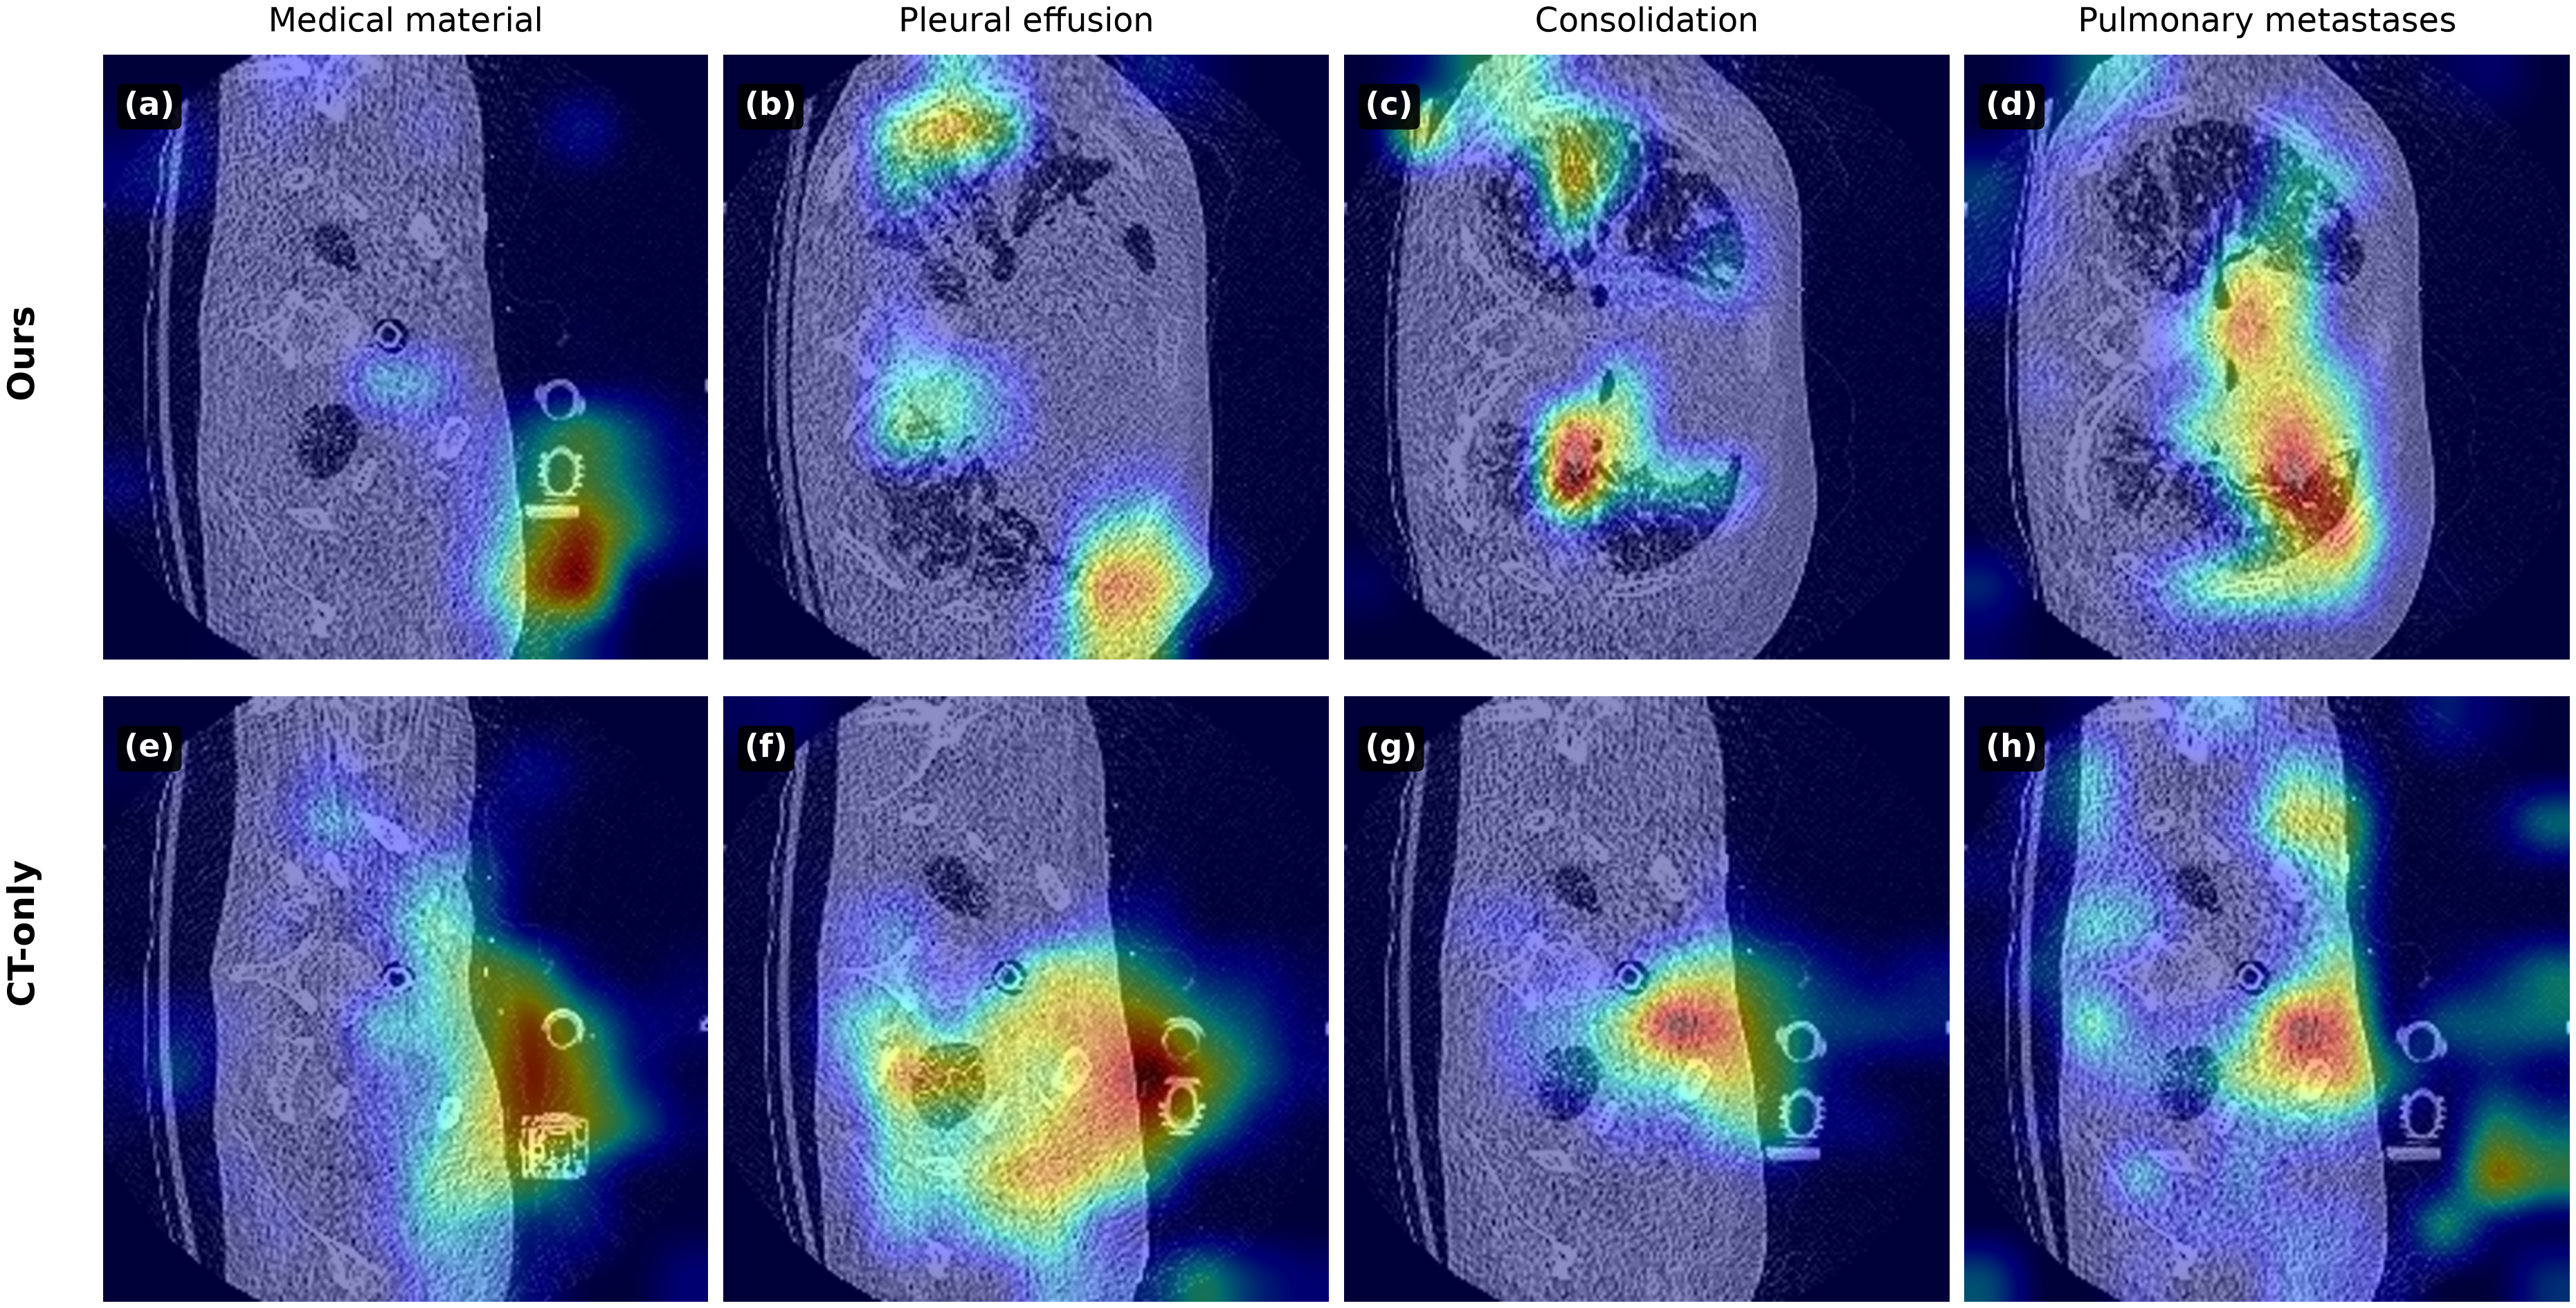
\includegraphics[width=\textwidth]{figures/pediatric_gradcam_case2.png}
\caption{Qualitative class-localization comparison in the ARC-CT Figure-2
layout. Top row (a--d): \ours{} supplied with the correct indication, age
band, and sex. Bottom row (e--h): the matched CT-only control. Columns show
medical material, pleural effusion, consolidation, and pulmonary metastases.
All four findings are ground-truth positive for this study. Warmer colors
indicate regions with greater influence on the corresponding model score.}
\label{fig:pediatric-gradcam}
\end{figure*}

\section{Replication on the Historical Age-$\geq5$ Cohort}
\subsection{Matched three-seed comparison}
On the historical 1,507-study validation cohort, the metadata-conditioned
model improves three-seed macro AUROC from $0.7933\pm0.0017$ to
$0.8396\pm0.0015$ ($+0.0463$, Table~\ref{tab:main}). All three conditioned
seeds exceed 0.83 and each improves over its own seed-matched control
(Table~\ref{tab:pedsseeds}). The improvement is positive for all 23
pathologies (\Cref{tab:pedsclass}), with the largest gains for pneumothorax
($+0.164$), pulmonary metastases ($+0.137$), post-surgical or post-treatment
change ($+0.117$), pulmonary cysts ($+0.103$), and mosaic attenuation
($+0.096$). These are the findings whose prior probability is most strongly
shaped by the clinical history a pediatric indication typically carries.

The current pediatric Stage-1 and banded-age recipe independently reproduces
this result on the same age-$\geq5$ cohort. Its three conditioned seeds score
0.8370, 0.8393, and 0.8399 (mean $0.8387\pm0.0015$), compared with 0.8177,
0.8159, and 0.7813 for matched CT-only training (mean $0.8050\pm0.0205$).
The paired mean gain is therefore $+0.0338$. The near-identical absolute AUROC
of the historical Refined-C1 recipe (0.8396) and current recipe (0.8387),
despite different initialization and demographic encoding, supports
replication rather than dependence on one training implementation.

\begin{table}[t]
\centering
\caption{Historical age-$\geq5$ matched prompt-inference validation results
(macro AUROC, mean $\pm$ SD over three seeds, $N=1,507$). These are not
independent test estimates.}
\label{tab:main}
\resizebox{\columnwidth}{!}{%
\begin{tabular}{@{}lccc@{}}
\toprule
Cohort & CT-only & \ours{} & $\Delta$ \\
\midrule
Age $\geq5$, 23 labels & 0.7933$\pm$.0017 & \best{0.8396$\pm$.0015} & \best{+0.0463} \\
\bottomrule
\end{tabular}}
\end{table}

\begin{table}[t]
\centering
\caption{Historical cohort: seeds and inference-time indication intervention
on the same trained checkpoints.}
\label{tab:pedsseeds}
\resizebox{\columnwidth}{!}{%
\begin{tabular}{@{}lrrrr@{}}
\toprule
Arm & Seed 0 & Seed 1 & Seed 2 & Mean \\
\midrule
CT-only & 0.7934 & 0.7950 & 0.7916 & 0.7933 \\
\ours, correct indication & \best{0.8386} & \best{0.8414} & \best{0.8389} & \best{0.8396} \\
\ours, indication blanked & 0.8111 & 0.8091 & 0.8074 & 0.8092 \\
\ours, indication shuffled & 0.7980 & 0.7967 & 0.7934 & 0.7960 \\
\bottomrule
\end{tabular}}
\end{table}

\subsection{Consistency across age}
The gain is also positive in every age stratum of the historical cohort
(Table~\ref{tab:age}), including the 5--10-year bin where CT-only performance
is lowest (0.7451 to 0.7904). The historical cohort extends above 18 years
because the source institution images young adults with childhood-onset
disease. Gains in those strata are of the same size as in children.

\begin{table}[t]
\centering
\caption{Historical cohort performance by age. Only eligible classes enter
each stratum's macro AUROC.}
\label{tab:age}
\resizebox{\columnwidth}{!}{%
\begin{tabular}{@{}lrrrr@{}}
\toprule
Age & $N$ & Classes & CT-only & \ours{} ($\Delta$) \\
\midrule
5--10 & 252 & 15 & 0.7451 & \best{0.7904} (+.0452) \\
10--18 & 768 & 23 & 0.7995 & \best{0.8440} (+.0445) \\
18--25 & 402 & 20 & 0.7729 & \best{0.8190} (+.0461) \\
25+ & 85 & 15 & 0.7615 & \best{0.8050} (+.0435) \\
All $<18$ & 1,020 & 23 & 0.7979 & \best{0.8412} (+.0433) \\
All $\geq18$ & 487 & 23 & 0.7841 & \best{0.8325} (+.0483) \\
\midrule
Pooled & 1,507 & 23 & 0.7933 & \best{0.8396} (+.0463) \\
\bottomrule
\end{tabular}}
\end{table}

\subsection{Completed historical age-$\geq5$ current-recipe ablations}
Every current-recipe arm with a completed evaluation on the historical
validation split is listed in \Cref{tab:peds-ge5-complete}. Unfinished arms are
kept in the experiment registry rather than displayed as empty paper rows.

\IfFileExists{generated/peds23_ge5_ablation.tex}{%
  \begingroup\renewcommand{\subsection}[1]{}%
  % Auto-generated historical pediatric ablation table.
\subsection{Completed historical age-$\geq5$ current-recipe ablations}
\begin{table*}[t]
\centering
\caption{Completed current-recipe age-$\geq5$ 23-target ablations on the same historical validation split. Global denotes the conditioned/fused prompt readout; arms without a completed evaluation are omitted.}
\label{tab:peds-ge5-complete}
\begin{tabular}{@{}lrrrrr@{}}
\toprule
Arm & Global AUC & General AUC & Global F1 & Global accuracy & Global precision \\
\midrule
Full model, three-seed mean & 0.8387 & 0.8143 & 0.3644 & 0.8675 & 0.5082 \\
CT-only, three-seed mean & 0.8050 & 0.8050 & 0.3303 & 0.8729 & 0.5174 \\
\midrule
Full current model, seed 0 & 0.8370 & 0.8076 & 0.3134 & 0.8695 & 0.5334 \\
Full current model, seed 1 & 0.8393 & 0.8167 & 0.3400 & 0.8745 & 0.4924 \\
Full current model, seed 2 & 0.8399 & 0.8185 & 0.4397 & 0.8586 & 0.4987 \\
CT-only, seed 0 & 0.8177 & 0.8177 & 0.3738 & 0.8776 & 0.5820 \\
CT-only, seed 1 & 0.8159 & 0.8159 & 0.3514 & 0.8792 & 0.5517 \\
CT-only, seed 2 & 0.7813 & 0.7813 & 0.2657 & 0.8617 & 0.4185 \\
Indication dropout 0.4 & 0.8216 & 0.7882 & 0.3314 & 0.8512 & 0.4987 \\
C1 off & 0.8103 & 0.7893 & 0.2896 & 0.8016 & 0.3982 \\
Indication conditioning only & 0.8204 & 0.7883 & 0.3591 & 0.8152 & 0.3997 \\
Demographic conditioning only & 0.8085 & 0.7890 & 0.3874 & 0.8298 & 0.4060 \\
Standard negative prompts & 0.8201 & 0.7767 & 0.3348 & 0.8257 & 0.4523 \\
Auxiliary ctx\_cls & 0.8243 & 0.7880 & 0.3781 & 0.8391 & 0.4762 \\
Indication-loss weight 1 & 0.8200 & 0.7862 & 0.3520 & 0.8173 & 0.4350 \\
Indication-loss weight 4 & 0.8229 & 0.7893 & 0.3634 & 0.8359 & 0.4199 \\
Qwen region text & 0.8206 & 0.7877 & 0.4036 & 0.7958 & 0.3817 \\
One global query & 0.8221 & 0.7879 & 0.3274 & 0.8478 & 0.3971 \\
Six global queries & 0.8238 & 0.7940 & 0.3294 & 0.8044 & 0.4276 \\
Augmentation off & 0.8223 & 0.7795 & 0.3587 & 0.8039 & 0.3523 \\
\bottomrule
\end{tabular}
\end{table*}
\begin{table}[t]
\centering
\caption{Available current-recipe indication interventions on the age-$\geq5$ cohort. Only completed evaluations are shown.}
\label{tab:peds-ge5-intervention-final}
\begin{tabular}{@{}llr@{}}
\toprule
Seed & Indication & AUROC \\
\midrule
0 & Correct & 0.8370 \\
0 & Blank & 0.8180 \\
1 & Correct & 0.8393 \\
1 & Blank & 0.8204 \\
1 & Shuffled & 0.8107 \\
2 & Correct & 0.8399 \\
\bottomrule
\end{tabular}
\end{table}
%
  \endgroup
}{%
  The complete historical age-$\geq5$ ablation render is pending.
}

\section{Does the Model Use the Correct Indication?}
\subsection{Inference-time intervention}
On the historical cohort, correct indications outperform blank and shuffled
indications by 3.04 and 4.36 AUROC points respectively
(Table~\ref{tab:pedsseeds}, Fig.~\ref{fig:intervention}). Shuffling preserves the marginal distribution of indication text and destroys
its pairing with the patient. It removes almost the entire gain over CT-only. The
model is therefore not benefiting from extra capacity or from the mere
presence of clinical language. It is reading the specific patient's
indication. The corresponding three-seed intervention on the frozen $<18$
split is queued and will be reported in the same form.

\begin{figure}[t]
\centering
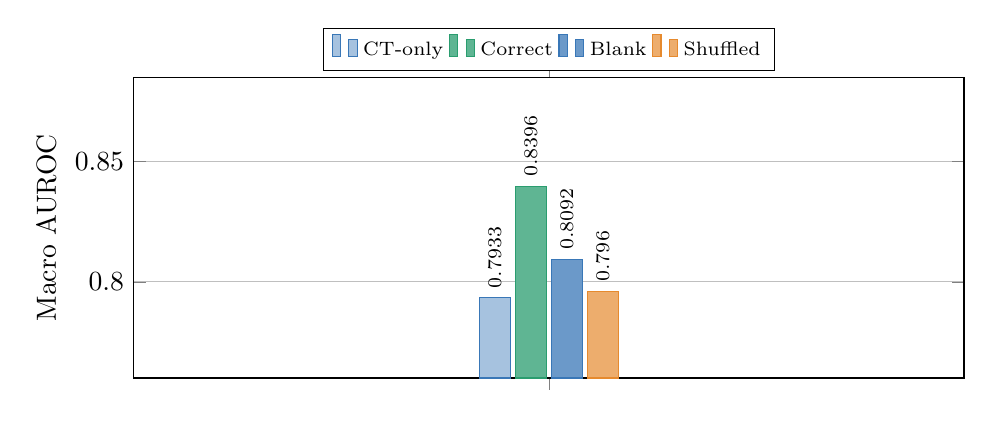
\begin{tikzpicture}
\begin{axis}[
  ybar,bar width=11pt,width=\columnwidth,height=5.4cm,
  ymin=0.76,ymax=0.885,ymajorgrids=true,
  enlarge x limits=0.6,
  symbolic x coords={Historical},xtick=data,xticklabels={},
  ylabel={Macro AUROC},
  legend style={at={(0.5,1.02)},anchor=south,legend columns=4,font=\scriptsize},
  nodes near coords,
  nodes near coords style={font=\scriptsize,rotate=90,anchor=west,
    /pgf/number format/fixed,/pgf/number format/precision=4}
]
\addplot[fill=ctblue!45,draw=ctblue] coordinates {(Historical,0.7933)};
\addplot[fill=ctxgreen!75,draw=ctxgreen] coordinates {(Historical,0.8396)};
\addplot[fill=ctblue!75,draw=ctblue] coordinates {(Historical,0.8092)};
\addplot[fill=ctxorange!70,draw=ctxorange] coordinates {(Historical,0.7960)};
\legend{CT-only,Correct,Blank,Shuffled}
\end{axis}
\end{tikzpicture}
\caption{Indication intervention on the same trained checkpoints, historical
age-$\geq5$ cohort ($N=1,507$, three-seed means). Blanking removes two-thirds
of the gain over CT-only. Shuffling removes nearly all of it.}
\label{fig:intervention}
\end{figure}

\subsection{How predictive is metadata without the CT?}
Table~\ref{tab:metadata-only} reports no-CT controls on the frozen $<18$ test
split. Age and sex alone are near chance (0.5064). Indication text alone,
however, reaches 0.7860 macro AUROC, \emph{higher than the matched CT-only
model's 0.7687}. Adding demographics to the indication adds only 0.0007. Two
consequences follow. First, on this cohort the clinical text is a stronger
single predictor than the image, which is itself a finding about pediatric
indications. Second, beating CT-only is not sufficient evidence of
multimodal fusion. The model must beat the text-only control as well. It does:
the full model's 0.8268 exceeds the indication-only head by 0.0408 and the
CT-only model by 0.0581, i.e., it uses both sources.

\begin{table}[t]
\centering
\caption{No-CT controls on the frozen $<18$ test split ($N=1,273$). AUROC is
mean $\pm$ SD over three linear-head seeds. AUPRC is the three-seed mean.}
\label{tab:metadata-only}
\resizebox{\columnwidth}{!}{%
\begin{tabular}{@{}lcc@{}}
\toprule
Input & Macro AUROC & Macro AUPRC \\
\midrule
Age + sex (no CT) & $0.5064\pm0.0065$ & 0.1578 \\
Indication (no CT) & $0.7860\pm0.0003$ & 0.3792 \\
Indication + age + sex (no CT) & $0.7867\pm0.0010$ & 0.3801 \\
\midrule
CT-only (image only) & $0.7687$ & 0.3592 \\
\ours{} (image + metadata) & $\best{0.8268}$ & \best{0.4616} \\
\bottomrule
\end{tabular}}
\end{table}

\subsection{Explicit terminology in the indication}
A conservative audit found that at least one positive target was explicitly
named in the indication for 1,064/4,320 (24.6\%) training, 169/748 (22.6\%)
development, and 330/1,273 (25.9\%) test studies. This heuristic cannot
distinguish a suspected from a confirmed diagnosis, so it is not by itself
evidence of leakage. Stratifying on it is informative nonetheless
(Table~\ref{tab:u18-mention-strata-snapshot}): the conditioned model improves
over CT-only both when the target is explicitly named (0.6694 to 0.7153) and
when it is not (0.7692 to 0.8249). The gain in the \emph{unflagged} majority is
larger than in the flagged minority, which is the opposite of what a lexical
shortcut would produce. Notably, absolute AUROC is lower in the flagged
stratum for both models: studies whose indication already names a finding are
harder, not easier, presumably because they are enriched for ambiguous
follow-up examinations.

\section{Pediatric Benchmark of Released Chest-CT Models}
\subsection{Why a local benchmark is necessary}
No published pediatric chest-CT benchmark exists, and the adult CT-RATE
leaderboard cannot be assumed to transfer. We therefore evaluated every
reproducible comparison method on the historical 1,507-study cohort with the
identical 23-label file, the identical metric code, and patient-grouped
bootstrap intervals (Table~\ref{tab:pedsbench}). Methods were assigned their
own published readout: GreenRFM's supervised head, MPS-CT's and CT-CLIP's
prompt softmax, and so on. For methods with multiple saved checkpoints,
selection followed the same best-of-$N$ validation rule our own models use.
This changed both affected baselines by at most 0.001 relative to their final
checkpoints. Four further methods reported on CT-RATE could not be measured because their
releases lack code, weights, a training entry point, or a license. Those
methods are BIUD, ViSD-Boost, BrgSA, and fVLM. We say so rather than importing
their adult numbers into a pediatric table.

\subsection{What the benchmark shows}
Three observations follow from Table~\ref{tab:pedsbench}.

\paragraph{Released adult models transfer poorly to children.}
CT-CLIP and its VocabFine variant fall to 0.5478 and 0.5339, barely above
chance, and H-LIP to 0.6916, from published adult AUROCs of 0.731 and 0.787.
For CT-CLIP this is not a readout artifact: sweeping all four prompt templates
shipped in its repository spans only 0.528--0.548, its image latents are not
degenerate (103 of 512 dimensions carry 90\% of variance), and a supervised
probe fitted on those latents reaches only 0.609. The limitation is
representational. A plausible mechanism is CT-CLIP's fixed 360\,mm in-plane
window: a small child occupies a much smaller fraction of that frame than the
adults it was trained on, and 29.5\% of our pediatric reconstructions exceed
the window and are cropped.

\paragraph{Pediatric adaptation helps every model, but unevenly.}
Adapting GreenRFM to the pediatric training split lifts it to 0.7477 and
MPS-CT to 0.6961. Both remain 9--14 points below \ours{} and 5--10 points below
our own CT-only control, which shares neither their architecture nor their
readout but does share the anatomy-routed initialization.

\paragraph{A 2-D encoder with a linear probe beats every volumetric model.}
A linear probe on frozen BiomedCLIP features reaches 0.7643, exceeding
GreenRFM, MPS-CT, and Merlin. Those features are 32 axial slices, mean-pooled,
with no three-dimensional context at all. Its per-class profile explains why: it is competitive on
findings legible in a single section and at chance (0.503) on lung nodules.
We do not read this as evidence against volumetric modeling. Our own
volumetric CT-only model at 0.7933 and full model at 0.8396 are well above it.
We read it as evidence that current volumetric \emph{pretraining}, as released,
buys less on pediatric CT than its adult rankings suggest, and that pediatric
performance must be measured rather than inherited.

\begin{table*}[t]
\centering
\begin{threeparttable}
\caption{Pediatric benchmark on the historical cohort (1,507 studies, 648
patients, 23 labels). All values are locally measured macro AUROC. Rows are
grouped by whether the method was adapted to the pediatric cohort, because a
pediatric-adapted model and an untrained transfer answer different questions.
Intervals are 1,000-sample bootstraps resampling patients.}
\label{tab:pedsbench}
\small
\begin{tabular}{@{}llccp{4.6cm}@{}}
\toprule
Method & Readout & AUROC & 95\% CI & Qualification \\
\midrule
\multicolumn{5}{@{}l}{\emph{Adapted to the pediatric cohort}}\\
\ours{} & conditioned prompt & \best{0.8396}\tnote{a} & seed SD only & three seeds, $\pm0.0015$ \\
Our CT-only & prompt & 0.7933\tnote{a} & seed SD only & matched three-seed control \\
BiomedCLIP, linear probe & supervised probe & 0.7643 & 0.7473--0.7803 & 2-D encoder, 32 axial slices, mean-pooled\tnote{b} \\
GreenRFM, local adaptation & supervised head & 0.7477 & 0.7310--0.7637 & best of 10 saved checkpoints (epoch 9) \\
Merlin, linear probe & supervised probe & 0.7144 & 0.6951--0.7313 & abdominal/pelvic CT model\tnote{c} \\
MPS-CT, local reproduction & zero-shot prompt & 0.6961 & 0.6840--0.7089 & best of 12 saved checkpoints (update 3,000) \\
GreenRFM, local reproduction & zero-shot prompt & 0.6620 & not estimated & prompt readout is ill-posed for this model\tnote{d} \\
\addlinespace
\multicolumn{5}{@{}l}{\emph{Released adult weights, no pediatric training}}\\
BiomedCLIP & zero-shot prompt & 0.6938 & 0.6695--0.7108 & fixed prompt pair, no tuning\tnote{b} \\
H-LIP & zero-shot prompt & 0.6916 & 0.6763--0.7048 & released CT-RATE weights \\
CT-CLIP & zero-shot prompt & 0.5478 & 0.5277--0.5670 & best of the four templates in the released code\tnote{e} \\
CT-CLIP VocabFine & zero-shot prompt & 0.5339 & 0.5113--0.5572 & second released CT-CLIP variant\tnote{e} \\
\bottomrule
\end{tabular}
\begin{tablenotes}[flushleft]\footnotesize
\item[a] Three-seed historical campaign (Table~\ref{tab:main}), reported with
seed standard deviation rather than a bootstrap interval. All other rows are
single trained models scored with identical metric code on the identical split.
\item[b] BiomedCLIP is a 2-D biomedical vision--language model applied
slice-wise with no inter-slice context. It reaches 0.503 (chance) on lung
nodule against 0.935 on pleural effusion. Its probe regularization was chosen
by patient-grouped cross-validation on the pediatric training split alone.
\item[c] Merlin is an abdominal/pelvic CT foundation model. This row is
out-of-domain on both body region and age, and its preprocessing resamples to
3\,mm slices.
\item[d] GreenRFM's contrastive objective uses unnormalized dot products at
fixed temperature, so per-volume embedding norm enters the cross-volume
ranking. Its published result is the supervised head above.
\item[e] The four CT-CLIP prompt templates span 0.528--0.548. A supervised
probe on CT-CLIP's own latents reaches 0.609.
\end{tablenotes}
\end{threeparttable}
\end{table*}

\section{Pediatric Report--CT Retrieval}
\subsection{Protocol}
Classification asks whether a model can name a finding. Retrieval asks whether
its image and report embeddings agree on \emph{which study} is which. We
therefore evaluated report$\rightarrow$image and image$\rightarrow$image
retrieval on the same 1,507-study cohort, with no retrieval-specific fitting
(\Cref{tab:pedsretrieval}). Report$\rightarrow$image is exact-match Recall@K:
each study's report queries all 1,507 volumes and only its own counts as a hit,
so chance is $K/N$. Every model encodes the byte-identical report string through its own text
tower at its own trained context length. That string is the impression-first
concatenation our own evaluator uses. Image$\rightarrow$image follows the
CT-CLIP/MPS-CT convention of mean label-set Jaccard between a query and its
top-$K$ retrieved studies, with one correction and one disclosure. The
correction: the query is excluded from its own gallery. The disclosure: the
evaluation script that prior work inherits from CT-CLIP does \emph{not}
exclude it, and also accumulates its running mean across successive $K$
without resetting, so the values those papers label ``MAP@K'' are inflated by
a guaranteed self-hit at $K{=}1$. We reproduced ARC-CT's published
71.3/61.7/54.3 to within 0.3 points from our own CT-RATE latents by applying
exactly that script. \Cref{tab:pedsretrieval} therefore reports the clean
metric as its headline and the inherited convention beside it, labelled, so
the pediatric numbers remain comparable to existing adult tables without
repeating their error.

\subsection{Findings}
Two structural facts shape the table. First, Refined C1 freezes the inherited
base and trains only the conditioned bank, so its metadata-free $z_{\mathrm{gen}}$
is identical to the seed-matched CT-only model's, verified to floating-point
noise on the stored latents. The metadata-free row is therefore shared. The
pediatric-specific question is whether conditioning on indication, age, and sex
changes retrieval. It is answered by the conditioned readouts, which use each
gallery study's own metadata and are labelled as not-equal-input. Second,
report$\rightarrow$image retrieval on children lands where it does on adults:
our $z_{\mathrm{gen}}$ reaches R@5/10/50/100 of 10.8/17.1/41.2/54.2, against
ARC-CT's published adult CT-RATE 11.4/18.0/40.4/52.1, so the image--report
alignment learned from pediatric reports is not weaker than the adult one.

The complete model sweeps the comparison set. \ours{} Refined C1 reading out
$\mathrm{norm}(z_{\mathrm{gen}}{+}z_{\mathrm{ind}})$ leads every prior method on
all ten columns of \Cref{tab:pedsretrieval}: 9.5/15.5/39.9/51.7 on
report$\rightarrow$image against the best baseline's 6.3/10.7/29.1/42.6, and
32.2/30.9/27.7 on clean image$\rightarrow$image Jaccard against 30.9/28.4/24.2.
The cross-model table carries only the full model and its matched CT-only
control, so it compares methods rather than our own readouts.
\Cref{tab:pedsretrieval-readout} separates the readouts. They split along an
interpretable axis rather than dominating each other. The metadata-free $z_{\mathrm{gen}}$
retrieves the \emph{exact} report best (10.8 at $K{=}5$), while the conditioned
$z_{\mathrm{ind}}$ retrieves the most \emph{label-similar} studies best (33.4 at
$K{=}5$, and highest at every $K$ under both conventions). Indication text
sharpens what a study is a case \emph{of} and blurs which particular report was
dictated for it. That is the behaviour expected if conditioning injects
clinical context rather than report-specific wording. The mixed readout sits
between the two by construction.

Among comparison methods, MPS-CT adapted to the pediatric cohort is a genuine
second (6.3/10.7/29.1/42.6). Released CT-CLIP and its VocabFine variant are at
chance (R@5 of 0.86 and 0.33 against $K/N{=}0.33$), the retrieval counterpart
of their near-chance classification transfer. GreenRFM is the instructive case:
even after pediatric adaptation its report$\rightarrow$image recall is at
chance (0.33/1.13/5.37/9.42), while its image$\rightarrow$image Jaccard (27.8
at $K{=}5$) shows the image space itself is informative. This is the same
mechanism that invalidated its prompt readout. A contrastive objective on
unnormalized dot products at fixed temperature does not learn a space in which
cosine similarity between a report and its volume is meaningful. That is also
why GreenRFM's own published results rest on its supervised head. Of the
released-weight rows, H-LIP is the strongest (3.6/5.8/14.9/22.4), above locally
adapted GreenRFM but below MPS-CT and every arm of ours. BiomedCLIP, which sees
the volume only as independent 2-D slices, reaches 1.9/3.3/11.8/17.4, and
Merlin, an abdominal--pelvic model applied to chest CT, is nearest chance at
1.0/1.7/6.2/10.9 while retaining a usable image space (21.8 Jaccard at
$K{=}5$).

One asymmetry is disclosed rather than corrected. Every model encodes the
identical impression-first string. Each uses its own tokenizer at its own
trained context length, and those lengths differ by an order of magnitude.
Merlin's 1,024 tokens truncate 5 of 1,507 reports. The 512 tokens of CT-CLIP
and H-LIP truncate about 107. The 128 tokens that GreenRFM and MPS-CT train
with truncate 1,368 of 1,507, or 91\%. The median report is 267 tokens long.
Extending their context would change the architecture we set out to reproduce,
so we report them at their published length and treat their
report$\rightarrow$image numbers as bounded by it. Image$\rightarrow$image
retrieval never touches the text encoder and is unaffected, which is consistent
with MPS-CT being a close second there while its recall is not.

\IfFileExists{generated/peds23_retrieval.tex}{%
  % Auto-generated by retr_make_table.py from PEDS_BENCH/retrieval/results; do not edit by hand.
\begin{table*}[t]\centering
\caption{Pediatric cross-modal retrieval on the historical cohort (1,507 studies, 648 patients), no retrieval-specific fitting. Report$\rightarrow$image is exact-match Recall@K over all 1,507 studies. Image$\rightarrow$image is mean label-set Jaccard of the top-$K$ retrieved studies (gallery = studies with $\geq$1 positive label): \emph{clean} excludes the query from its own gallery; \emph{Table-4 convention} reproduces the CT-CLIP evaluation script used by prior work, which includes the query and accumulates across $K$, and is shown only for comparability with published adult tables. Our arms are three-seed means; chance Recall@K is $K/N$.}
\label{tab:pedsretrieval}\small
\resizebox{\textwidth}{!}{%
\begin{tabular}{@{}lrrrrrrrrrr@{}}\toprule
 & \multicolumn{4}{c}{Report$\rightarrow$image R@K} & \multicolumn{3}{c}{Image$\rightarrow$image, clean} & \multicolumn{3}{c}{Image$\rightarrow$image, Table-4 conv.}\\
\cmidrule(lr){2-5}\cmidrule(lr){6-8}\cmidrule(lr){9-11}
Method & @5 & @10 & @50 & @100 & @5 & @10 & @50 & @5 & @10 & @50 \\ \midrule
\multicolumn{11}{@{}l}{\emph{Adapted to the pediatric cohort}}\\
\ours{} (full, metadata-conditioned)$^{\mathrm{m}}$ & 9.5$\pm$0.4 & 15.5$\pm$0.2 & 39.9$\pm$0.6 & 51.7$\pm$1.4 & \best{32.2$\pm$0.6} & \best{30.9$\pm$0.6} & \best{27.7$\pm$0.4} & \best{67.7} & \best{57.5} & \best{50.4} \\
\ours{} / CT-only control (metadata-free) & \best{10.8$\pm$0.6} & \best{17.1$\pm$0.1} & \best{41.2$\pm$0.4} & \best{54.2$\pm$1.2} & 31.7$\pm$0.2 & 30.4$\pm$0.3 & 27.5$\pm$0.1 & 67.4 & 57.2 & 50.1 \\
GreenRFM, local adaptation (epoch 9) & 0.3 & 1.1 & 5.4 & 9.4 & 27.8 & 26.2 & 23.4 & 66.0 & 54.9 & 47.4 \\
MPS-CT, local reproduction (update 3,000) & 6.3 & 10.7 & 29.1 & 42.6 & 30.9 & 28.4 & 24.2 & 67.3 & 56.5 & 48.8 \\
\multicolumn{11}{@{}l}{\emph{Released weights, no pediatric training}}\\
H-LIP & 3.6 & 5.8 & 14.9 & 22.4 & 23.7 & 22.6 & 20.8 & 64.2 & 52.7 & 45.0 \\
BiomedCLIP (2-D, slice-wise) & 1.9 & 3.3 & 11.8 & 17.4 & 25.3 & 23.8 & 21.0 & 64.9 & 53.5 & 45.8 \\
Merlin (abdominal) & 1.0 & 1.7 & 6.2 & 10.9 & 21.8 & 21.3 & 19.9 & 63.4 & 51.7 & 44.1 \\
CT-CLIP & 0.9 & 1.3 & 5.4 & 10.2 & 19.8 & 19.4 & 18.8 & 62.6 & 50.6 & 43.0 \\
CT-CLIP VocabFine & 0.3 & 0.9 & 3.7 & 6.7 & 20.8 & 20.0 & 19.1 & 62.9 & 51.0 & 43.4 \\
\midrule Chance ($K/N$) & 0.3 & 0.7 & 3.3 & 6.6 & -- & -- & -- & -- & -- & -- \\
\bottomrule\end{tabular}}
\vspace{1mm}\parbox{\textwidth}{\footnotesize $^{\mathrm{m}}$Uses each gallery study's own indication, age, and sex through the conditioned bank; not an equal-input comparison with the metadata-free rows, shown to test whether conditioning changes retrieval. Every model encodes the identical impression-first report string; each uses its own tokenizer at its own trained context length, which truncates long reports: ours 256 tokens; CT-CLIP 512 (107 of 1,507 truncated); VocabFine 512 (107 of 1,507 truncated); H-LIP 512 (106 of 1,507 truncated); GreenRFM 128 (1,368 of 1,507 truncated, 91\%); MPS-CT 128 (1,368 of 1,507 truncated, 91\%); BiomedCLIP 256 (846 of 1,507 truncated, 56\%); Merlin 1,024 (5 of 1,507 truncated). Single-model rows carry 1,000-draw patient-bootstrap intervals in the accompanying JSON.}
\end{table*}
\begin{table}[t]\centering
\caption{Readout ablation for \ours{} on the same pediatric retrieval task and the same stored latents as \Cref{tab:pedsretrieval}; three-seed means. The two tasks have opposite winners: the metadata-free readout retrieves the exact report best, the conditioned readout retrieves the most label-similar studies best.}
\label{tab:pedsretrieval-readout}\small
\resizebox{\columnwidth}{!}{%
\begin{tabular}{@{}lrrrr@{}}\toprule
Readout & R@5 & R@100 & Jaccard@5 & Jaccard@50 \\ \midrule
$z_{\mathrm{gen}}$, metadata-free (shared with CT-only) & \best{10.8$\pm$0.6} & \best{54.2$\pm$1.2} & 31.7$\pm$0.2 & 27.5$\pm$0.1 \\
$\mathrm{norm}(z_{\mathrm{gen}}{+}z_{\mathrm{ind}})$, full model$^{\mathrm{m}}$ & 9.5$\pm$0.4 & 51.7$\pm$1.4 & 32.2$\pm$0.6 & 27.7$\pm$0.4 \\
$z_{\mathrm{ind}}$, conditioned only$^{\mathrm{m}}$ & 8.0$\pm$1.0 & 47.2$\pm$1.1 & \best{33.4$\pm$0.7} & \best{28.0$\pm$0.6} \\
\bottomrule\end{tabular}}
\vspace{1mm}\parbox{\columnwidth}{\footnotesize $^{\mathrm{m}}$Uses each gallery study's own indication, age, and sex; not an equal-input comparison with the metadata-free row.}
\end{table}
%
}{%
  The retrieval table is pending. No numerical placeholders are treated as
  evidence.
}

\begin{figure*}[p]
\centering
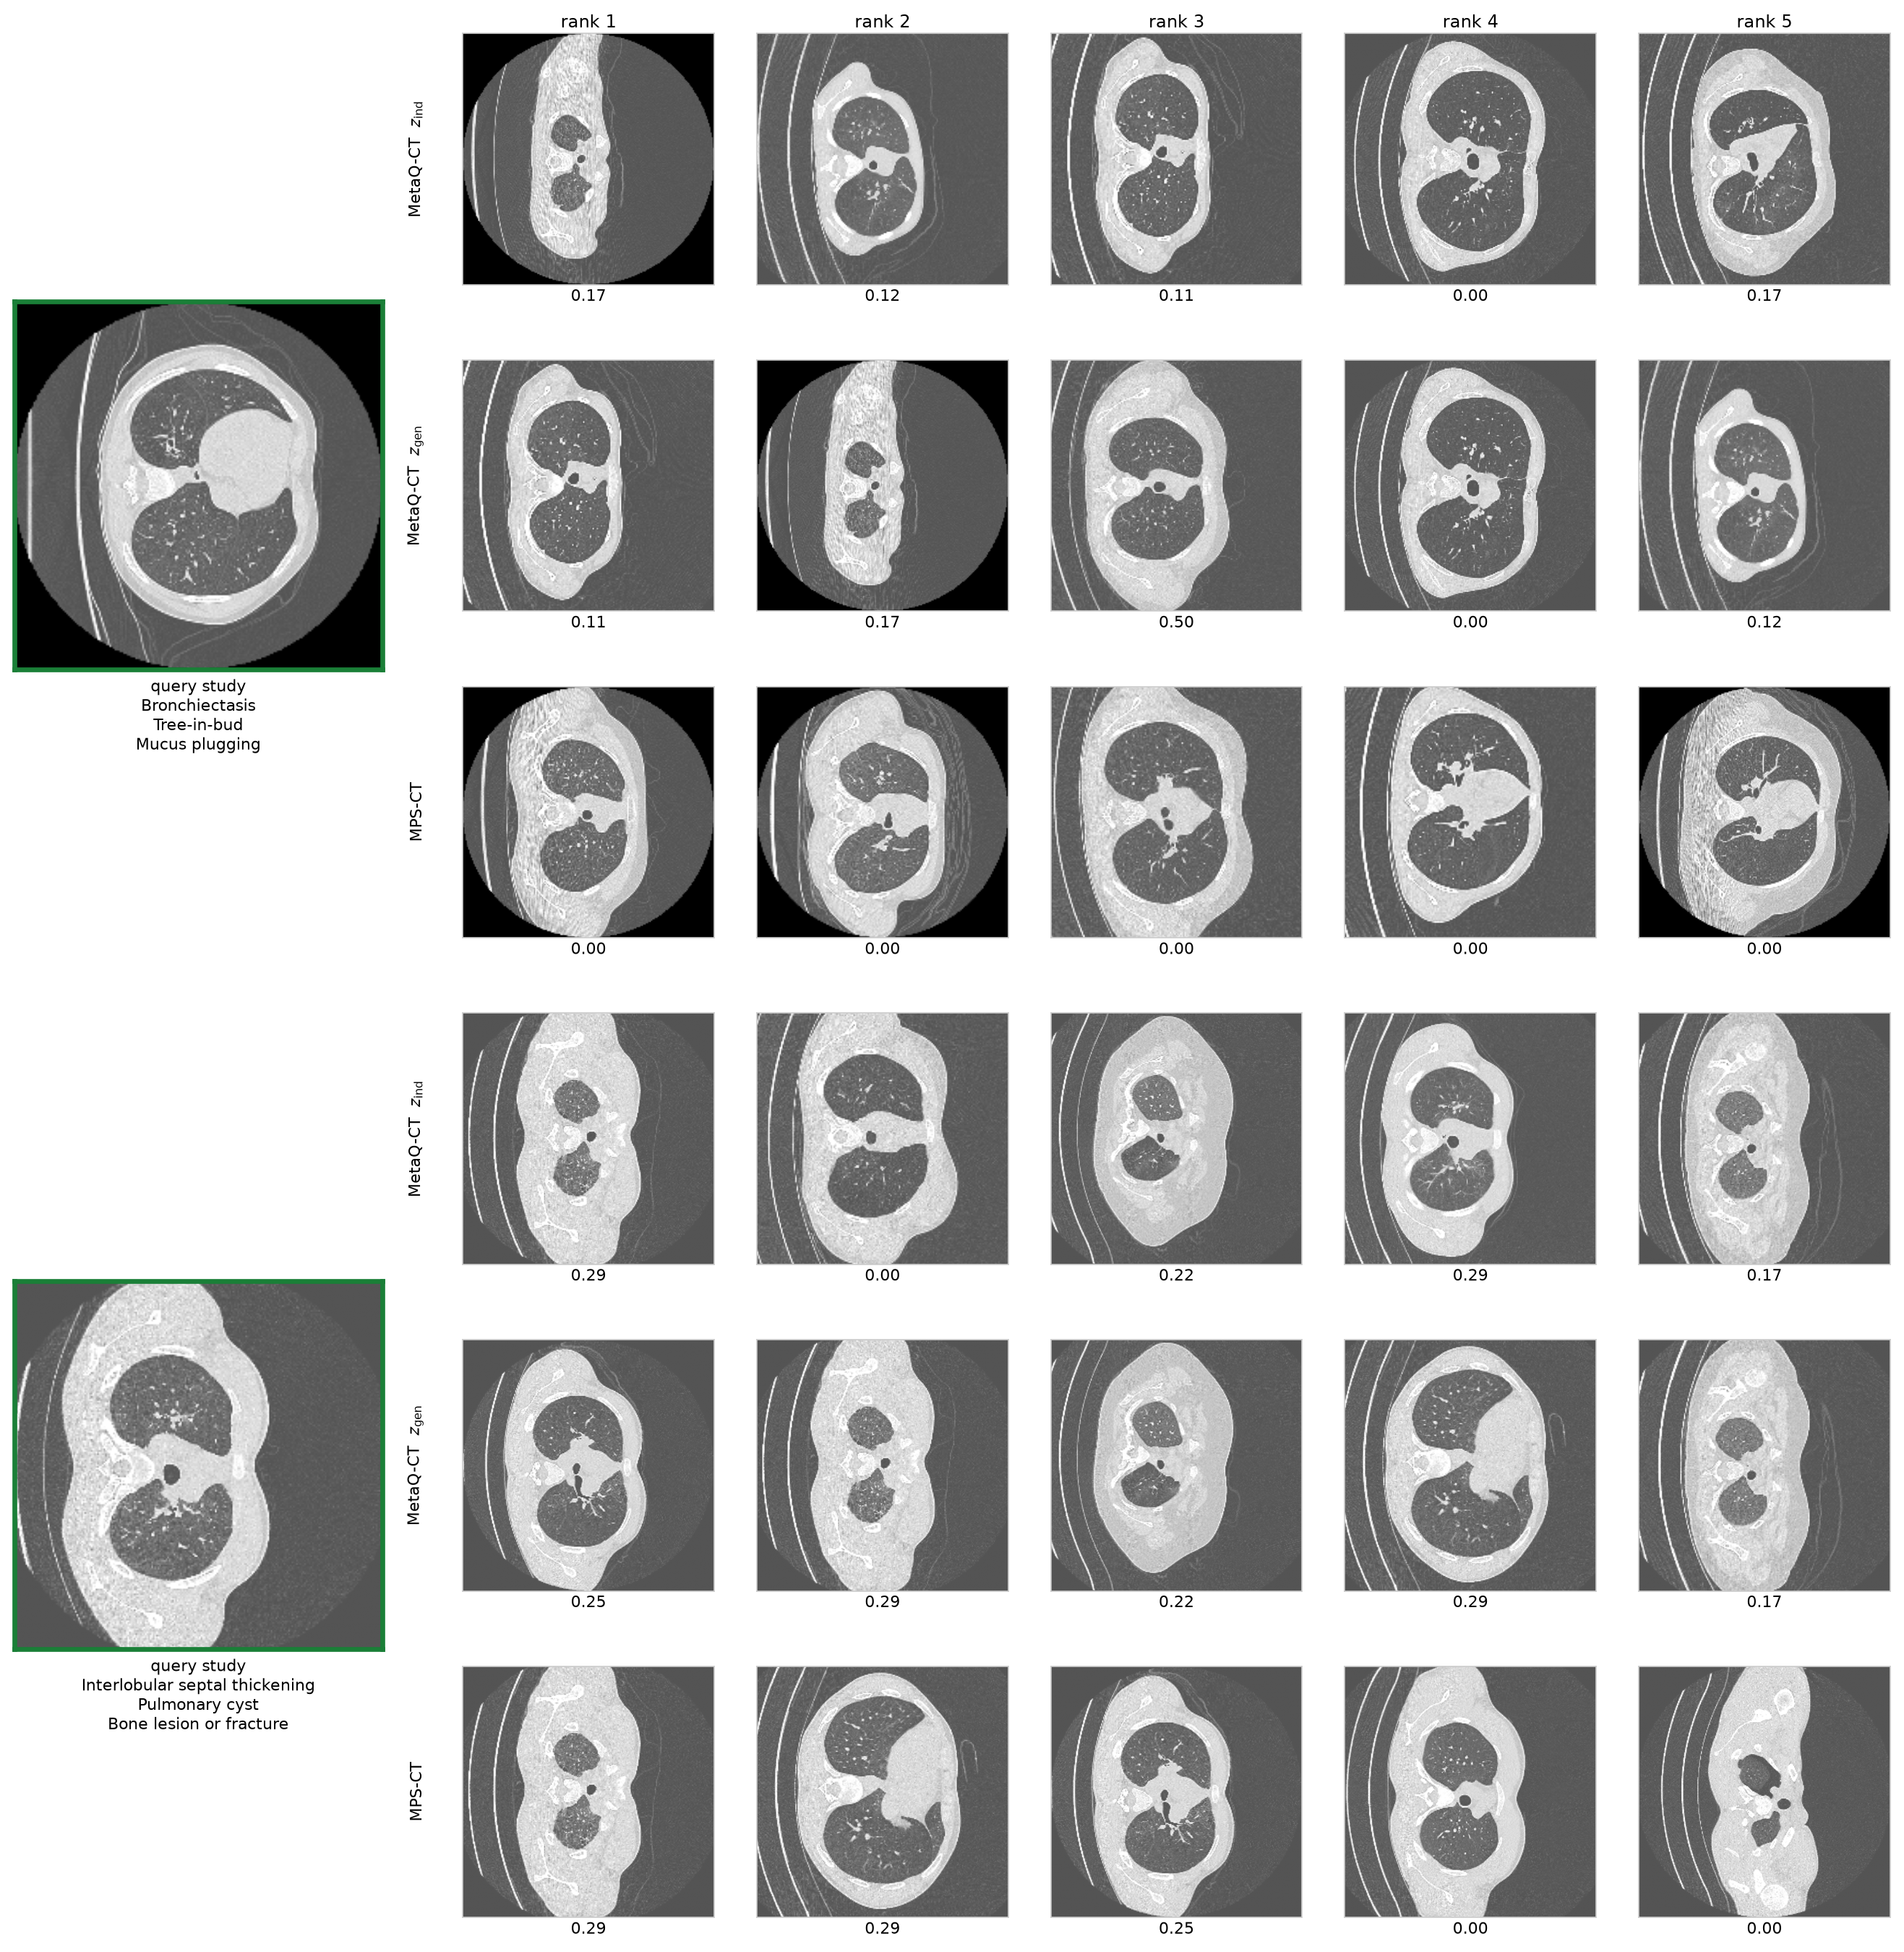
\includegraphics[width=\textwidth]{figures/peds_retrieval_i2i.png}
\caption{\textbf{Qualitative image$\rightarrow$image retrieval.} The query study
is on the left (green frame) with its ground-truth findings. Each row is one
method's top five by cosine similarity in that method's own embedding space,
with the query excluded from its own gallery. The number under each panel is the
label-set Jaccard against the query, the same quantity averaged in
\Cref{tab:pedsretrieval}. Queries were fixed without reference to any method's
scores: among test studies with exactly three positive findings whose field of
view frames the thorax, the two whose findings are rarest in the cohort. One
representative mid-thoracic axial slice is shown per study in a lung window.
That slice is the one with the most lung-density voxels in the central field.
Retrieval itself uses the whole volume. For the airway-disease query, MPS-CT returns
studies that are globally similar in appearance but share no label with the
query at any of the five ranks. This is the pediatric counterpart of the
globally-similar-but-pathologically-mismatched failure reported for
single-stage retrieval in prior work.}
\label{fig:peds-retrieval-i2i}
\end{figure*}

\begin{figure*}[p]
\centering
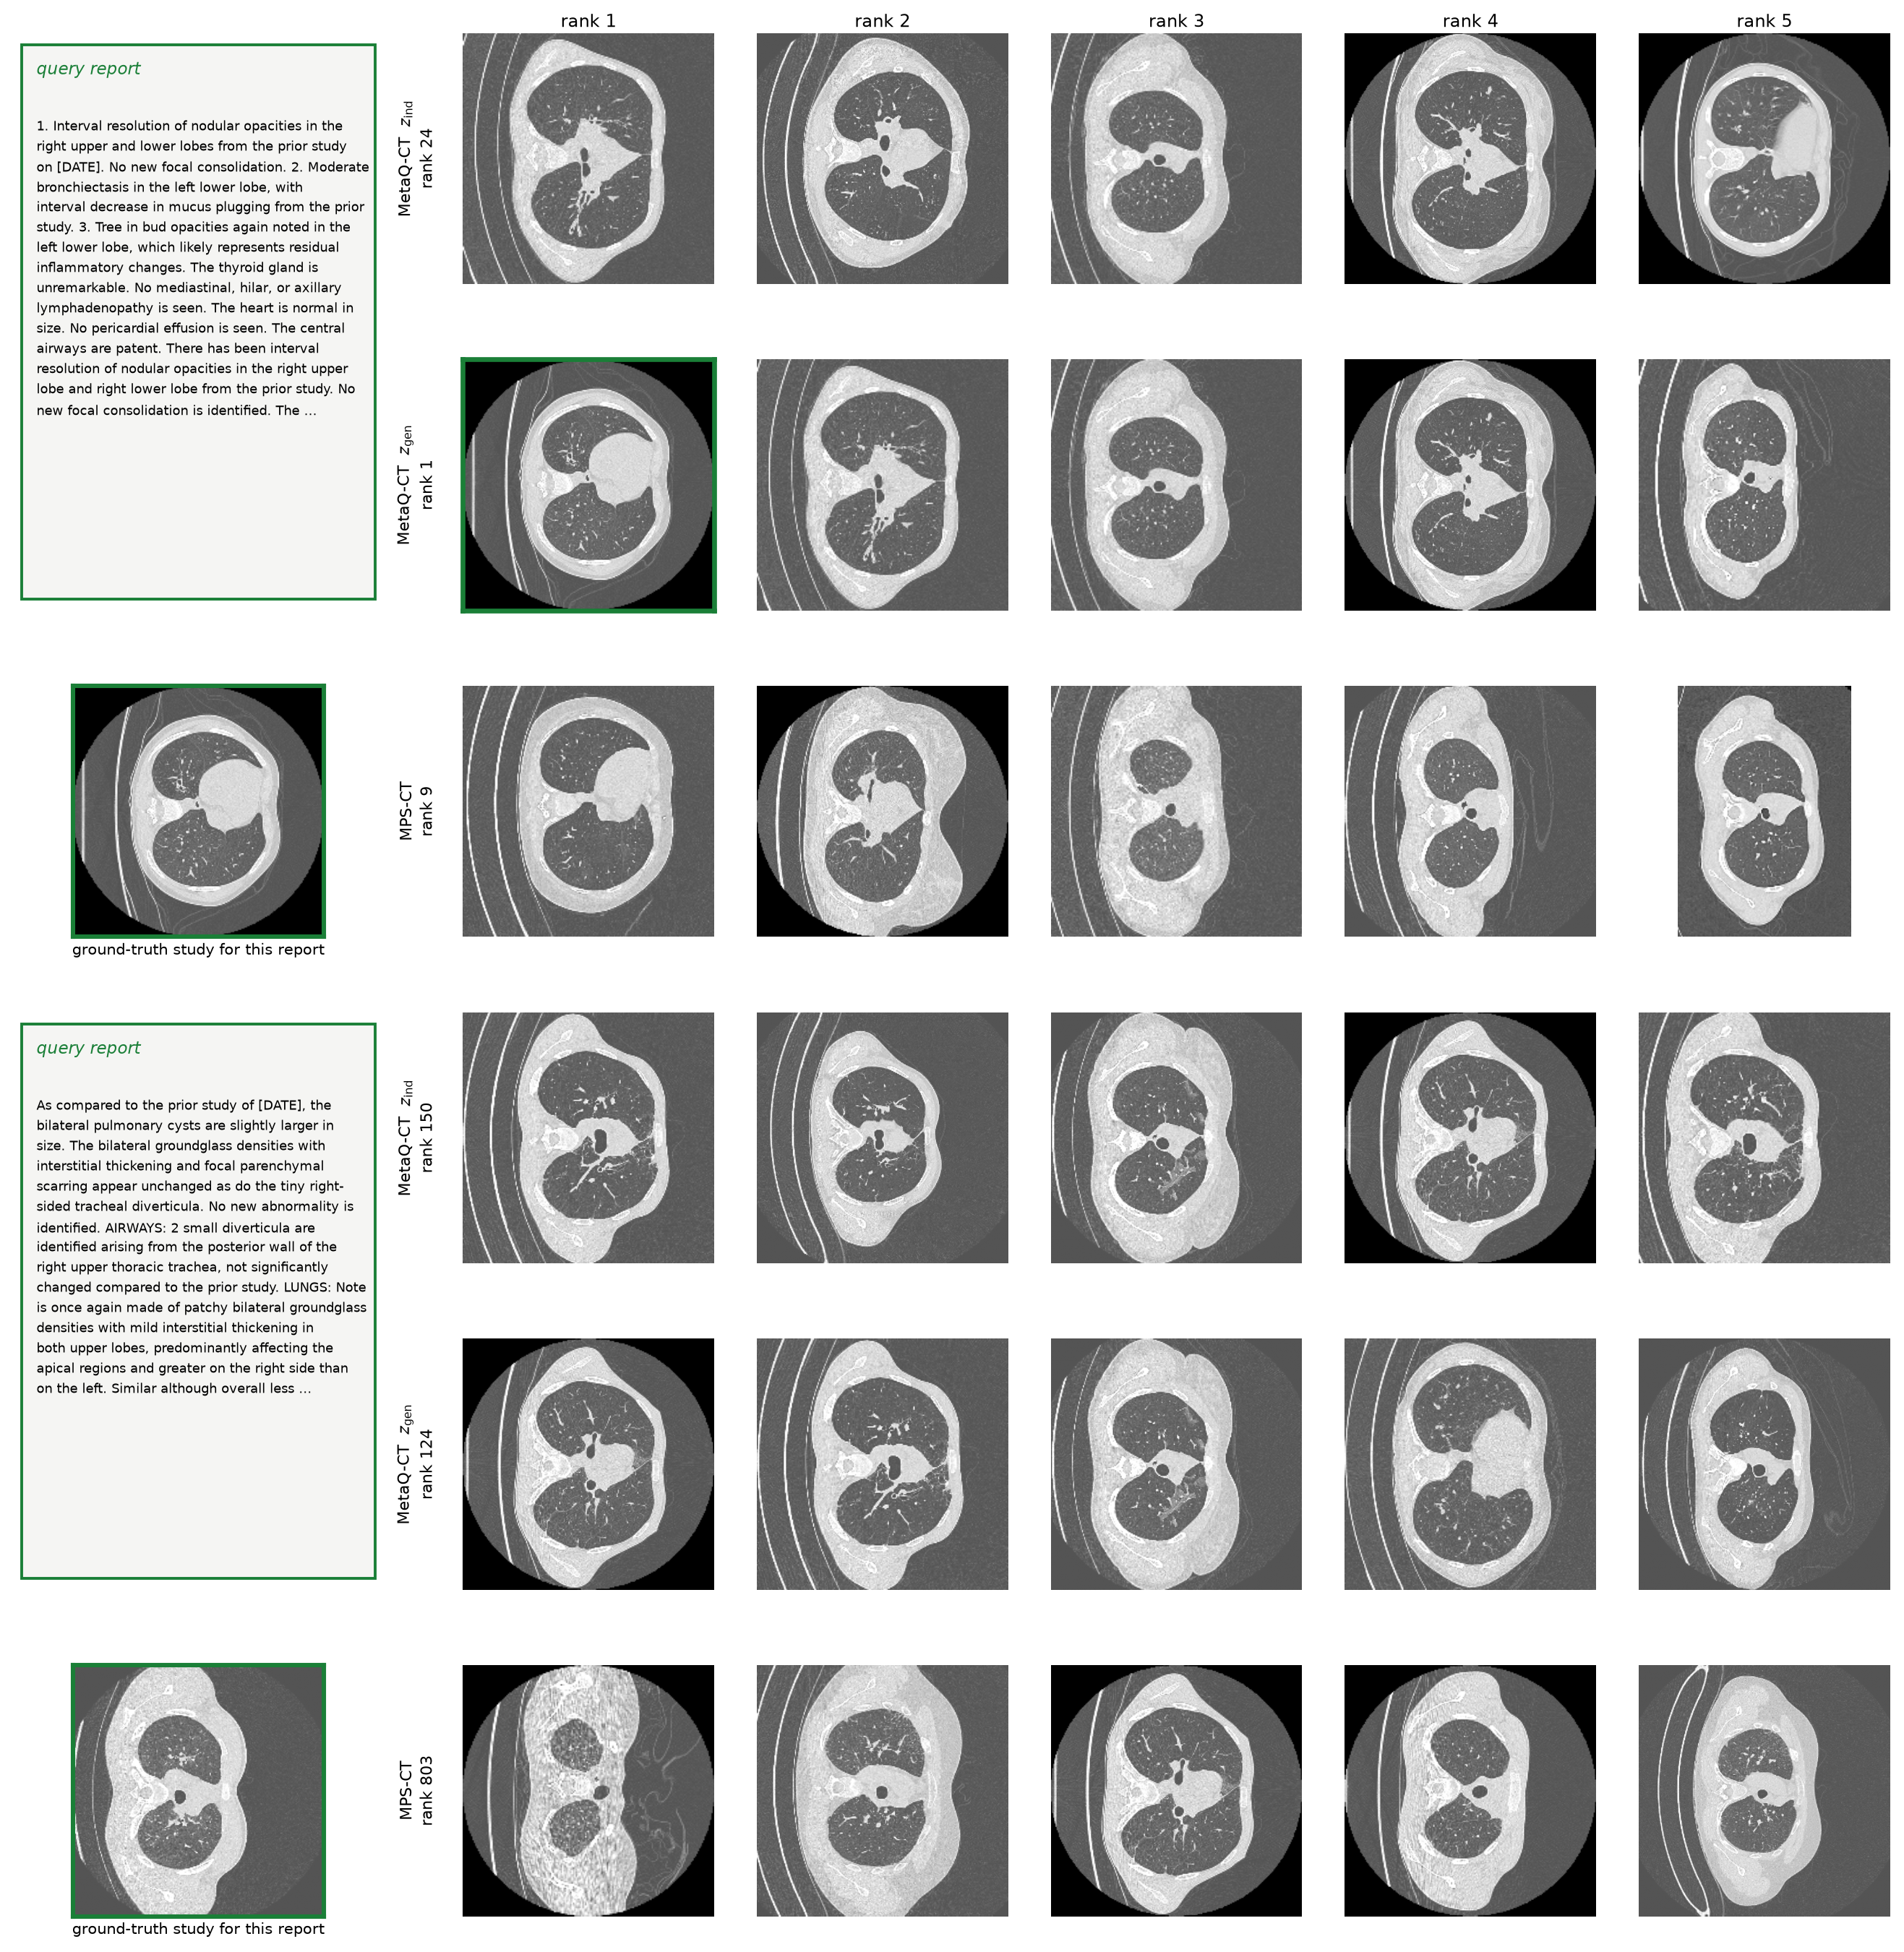
\includegraphics[width=\textwidth]{figures/peds_retrieval_r2i.png}
\caption{\textbf{Qualitative report$\rightarrow$image retrieval.} The query is
the impression-first report string, shown wrapped at the left with the study it
was dictated for beneath it. The queries are the same two studies as
\Cref{fig:peds-retrieval-i2i}. Each row is one method's top five volumes ranked
by cosine similarity to that report, and the row label gives the rank the
ground-truth study actually received out of 1,507. A green frame marks it when
it falls inside the top five. The upper query separates the two readouts in the
direction the aggregate numbers predict: the metadata-free $z_{\mathrm{gen}}$
places the correct study first, the conditioned $z_{\mathrm{ind}}$ places it
24th, and MPS-CT 9th. The lower query is a case no method solves (ranks 150,
124, and 803), included so the figure reports failures as well as successes.}
\label{fig:peds-retrieval-r2i}
\end{figure*}

\section{Is the Effect Specific to Pediatrics?}
The same architecture was trained and evaluated on the adult CT-RATE
benchmark, using the official validation split and the full 46,394-volume
training cache. It improves there too. On one final checkpoint, read from a
single forward pass, the image-only general prompt branch reaches 0.8733 macro
AUROC and the conditioned prompt branch reaches 0.8781 with the true
indication, a paired gain of $+0.0048$. With every indication blanked the same
branch reaches 0.8754. The mechanism is therefore not a pediatric artifact.

The causal picture differs sharply. Blanking removes 0.27 points of a
0.48-point adult gain. In children it removes most of a gain that is an order
of magnitude larger. Adult CT-RATE indications are frequently missing or
generic, so most of the adult gain arises from class-specific residual
adaptation rather than from indication semantics. Pediatric indications are
where patient-specific clinical context actually carries diagnostic
information, and that is where conditioning on it pays off. The adult numbers
above are a single checkpoint. Their three-seed replication and the
shuffled-indication control are registered in the companion adult paper.

\section{Discussion}
The pediatric improvement is large, seed-consistent, positive for 22 of 23
pathologies in the frozen snapshot and all 23 in the historical replication,
positive in every prespecified subgroup, replicated across two cohorts
and two training recipes, and nearly eliminated by assigning the wrong
indication. It survives the two controls most likely to expose a shortcut:
the model exceeds a text-only head that already reads the indication, and its
gain is larger on studies whose indication does \emph{not} name the finding.
The pattern supports a clinically plausible mechanism. Pediatric indications
are rich. They carry oncologic history, surgical context, transplant status,
and genetic diagnoses. They shift the prior for exactly the findings
whose per-class gains are largest: metastases, post-treatment change, cysts,
pneumothorax. The design lets that prior act on the pathology slots it
concerns while leaving the general representation untouched.

Two further results have practical weight for anyone building pediatric CT
models. The age factorial shows that a conditioned model should be trained on
the full 0--18 range: only the CT-only baseline benefits from excluding the
youngest children. The benchmark also shows that adult CT foundation models,
as released, are not a safe starting point for pediatric deployment. Two of
them are near chance, and a generic 2-D encoder with a linear layer beats the
volumetric models we could reproduce.

\section{Limitations}
The cohort is retrospective and from a single children's hospital. The
primary frozen $<18$ results are from an interim checkpoint snapshot taken
while training continued. The converged three-seed comparison, the $<18$
indication intervention, and the completed component matrix are queued and
will replace the interim tables through the same generated fragments. The
frozen test pool, while MRN-disjoint and never used for selection in this
campaign, was visible during earlier exploratory analyses, so we do not claim
a prospective test. The historical replication cohort is a held-out
validation set, not an independent test. The conditioned branch improves
discrimination but is not yet better calibrated than CT-only, so a deployed
version would require post-hoc calibration. Labels are report-derived. Two of
1,507 historical validation volumes are stored non-axially or carry
inconsistent header spacing and are therefore anatomically wrong input for
every row of the benchmark, including ours. At 0.13\% they do not move a macro
AUROC but are noted for completeness. Benchmark rows are local measurements
rather than published pediatric results. Several are not architecture-matched,
four methods could not be reproduced at all, and a pediatric fine-tune of
CT-CLIP remains outstanding. Report-generation metrics and blinded radiologist
review are not part of this paper.

\section{Conclusion}
Conditioning a volumetric CT Q-Former on indication, age, and sex through
pathology-specific queries yields a reproducible 5.8-point macro-AUROC gain on
a frozen MRN-disjoint pediatric test split and a 4.6-point gain on a second
pediatric cohort, positive in every age, sex, year, and site subgroup.
Counterfactual interventions and no-CT controls show that the gain comes from
reading the correct patient's clinical context and fusing it with the image,
not from text alone or from added capacity. A locally measured benchmark shows
that adult chest-CT foundation models transfer poorly to children and that
pediatric performance must be measured directly. Together these findings
argue for clinical context as an explicit, auditable input to pediatric
medical vision--language models.

\clearpage
\appendix
\section{Complete Per-Class Results}
The frozen $<18$ per-class results are in
Table~\ref{tab:u18-per-class-snapshot} (generated). The matched historical
age-$\geq5$ per-class results are in \Cref{tab:pedsclass}.

\begin{table*}[t]
\centering
\caption{Historical age-$\geq5$ per-class AUROC, averaged over three seeds
($N=1,507$).}
\label{tab:pedsclass}
\resizebox{\textwidth}{!}{%
\begin{tabular}{@{}lrrr@{\hspace{0.8cm}}lrrr@{}}
\toprule
Pathology & CT-only & \ours{} & $\Delta$ & Pathology & CT-only & \ours{} & $\Delta$ \\
\midrule
Medical material & .8562 & .9024 & +.0463 & Peribronchial thickening & .8236 & .8431 & +.0195 \\
Cardiomegaly & .9441 & .9528 & +.0088 & Consolidation & .9241 & .9286 & +.0045 \\
Pericardial effusion & .7880 & .8125 & +.0245 & Bronchiectasis & .9101 & .9250 & +.0149 \\
Lymphadenopathy & .8042 & .8163 & +.0121 & Interlobular septal thickening & .8462 & .8828 & +.0366 \\
Atelectasis & .7126 & .7233 & +.0107 & Post-surgical/treatment change & .7485 & .8658 & +.1174 \\
Lung nodule & .6507 & .6937 & +.0431 & Pulmonary metastases & .6662 & .8036 & +.1374 \\
Lung opacity & .8148 & .8329 & +.0181 & Tree-in-bud & .8280 & .8737 & +.0457 \\
Pulmonary fibrotic sequela & .7512 & .7764 & +.0252 & Pulmonary cyst & .7523 & .8548 & +.1025 \\
Pleural effusion & .9729 & .9754 & +.0025 & Mass/neoplasm & .8496 & .8680 & +.0184 \\
Mosaic attenuation & .7413 & .8368 & +.0956 & Mucus plugging & .8622 & .9014 & +.0392 \\
Pleural thickening/nodule & .6607 & .6819 & +.0212 & Bone abnormality & .5789 & .6348 & +.0559 \\
Pneumothorax & .7606 & .9245 & +.1639 & \textbf{Macro mean} & \textbf{.7933} & \textbf{.8396} & \textbf{+.0463} \\
\bottomrule
\end{tabular}}
\end{table*}

\section{Primary-Cohort Label Distribution}
Per-study prevalence of each of the 23 targets in the three splits of the
primary $<18$ cohort is given in \Cref{tab:label-prevalence}. Prevalence
ranges from 2.3\% (pneumothorax) to 42.7\% (medical material), and the
development split tracks the training distribution because it was selected to
do so, while the test pool was fixed independently.

\begin{table*}[t]
\centering
\caption{Per-study target prevalence (\%) in the primary $<18$ cohort. The
MRN-grouped development split was selected to preserve the multilabel
distribution. The test pool was fixed independently.}
\label{tab:label-prevalence}
\resizebox{\textwidth}{!}{%
\begin{tabular}{@{}lrrr@{\hspace{0.8cm}}lrrr@{}}
\toprule
Target & Train & Dev. & Test & Target & Train & Dev. & Test \\
\midrule
Medical material & 42.7 & 40.4 & 42.0 & Bronchiectasis & 10.8 & 11.9 & 8.1 \\
Cardiomegaly & 2.8 & 3.1 & 2.3 & Interlobular septal thickening & 5.6 & 5.3 & 6.0 \\
Pericardial effusion & 4.3 & 4.7 & 3.5 & Post-surgical or post-treatment change & 30.4 & 32.6 & 30.8 \\
Lymphadenopathy & 7.6 & 6.3 & 7.5 & Pulmonary metastases & 5.6 & 5.5 & 6.0 \\
Atelectasis & 34.4 & 34.5 & 35.1 & Tree-in-bud & 7.9 & 7.9 & 7.1 \\
Lung nodule & 48.8 & 48.5 & 49.6 & Pulmonary cyst & 5.3 & 4.7 & 3.9 \\
Lung opacity & 31.7 & 29.7 & 33.5 & Mass or neoplasm & 2.2 & 2.4 & 2.6 \\
Pulmonary fibrotic sequela & 17.9 & 18.4 & 18.5 & Mucus plugging & 4.5 & 4.7 & 3.5 \\
Pleural effusion & 3.8 & 4.0 & 3.8 & Pleural thickening or nodule & 9.8 & 9.5 & 11.5 \\
Mosaic attenuation pattern & 15.2 & 15.6 & 14.5 & Bone lesion or fracture & 11.1 & 11.1 & 14.1 \\
Peribronchial thickening & 15.0 & 15.4 & 13.2 & Pneumothorax & 2.3 & 1.9 & 2.0 \\
Consolidation & 6.5 & 5.1 & 6.0 & & & & \\
\bottomrule
\end{tabular}}
\end{table*}

\section{Benchmark Reproducibility Notes}
Every benchmark row was re-derived from its own saved prediction file and
verified against the labels file: class order identical, zero mismatched
label rows, 1,507 studies from 648 patients in every case. Comparison models
were run with their own released code and unmodified architectures. The only
edits were to data loading and, for CT-CLIP's trainer, making a hard-coded
18-class diagnostic list overridable so it would not crash on a 23-class
cohort. Pediatric volumes are stored in Hounsfield units with the rescale
carried in the NIfTI header. All pipelines were checked to apply it exactly
once. The primary model starts from Kinetics initialization and pediatric
Stage-1 adaptation, with no CT-RATE scan or adult ARC-CT checkpoint entering
its pediatric optimization. Comparison methods instead follow the
initialization prescribed by their own releases: CT-CLIP, H-LIP, Merlin, and
BiomedCLIP start from released adult weights, while rows labelled ``local
adaptation'' or ``local reproduction'' are additionally fitted on the
pediatric training split. This initialization difference is stated explicitly
because it answers a transfer question rather than a from-scratch architecture
comparison.

\bibliographystyle{plain}
\bibliography{references}

\end{document}
